%  LaTeX support: latex@mdpi.com 
%  For support, please attach all files needed for compiling as well as the log file, and specify your operating system, LaTeX version, and LaTeX editor.

% Primary target: MDPI Journal of Imaging.  The file also has a standalone fallback so
% it can be compiled before the MDPI Definitions/ folder is supplied.
%=================================================================

%\documentclass[journal,article,submit,moreauthors]

\IfFileExists{Definitions/mdpi.cls}{%
  %\documentclass[mathematics,article,submit,pdftex,moreauthors]
  \documentclass[jimaging,article,submit,pdftex,moreauthors]
  {Definitions/mdpi}
  \newif\ifmdpiclass\mdpiclasstrue
}{%
  \documentclass[11pt,a4paper]{article}
  \newif\ifmdpiclass\mdpiclassfalse
}
% For posting an early version of this manuscript as a preprint, you may use "preprints" as the journal. Changing "submit" to "accept" before posting will remove line numbers.
\ifmdpiclass
\else
  \usepackage[a4paper,margin=25mm]{geometry}
  \usepackage{graphicx}
  \usepackage{booktabs}
  \usepackage{tabularx}
  \usepackage{array}
  \usepackage{float}
  \usepackage{amsmath,amssymb}
  \usepackage{enumitem}
  \usepackage[numbers,sort&compress]{natbib}
  \usepackage{url}
  % The standalone fallback avoids a hard dependency on hyperref so it can be
  % compiled on minimal TeX installations. The MDPI class supplies hyperlinks.
  \providecommand{\href}[2]{#2}
\fi

%=================================================================
% REVISION HIGHLIGHTING
% Text added or changed in response to the reviewers is shown in blue.
% Comment out the next line to remove the blue highlighting (clean version).
\def\ShowRevisions{}
%=================================================================
\RequirePackage{xcolor}
\RequirePackage{placeins}
\ifdefined\ShowRevisions
  \DeclareRobustCommand{\rev}[1]{\textcolor{blue}{#1}}
  \newcommand{\revbegin}{\begingroup\color{blue}}
\else
  \DeclareRobustCommand{\rev}[1]{#1}
  \newcommand{\revbegin}{\begingroup}
\fi
\newcommand{\revend}{\ifhmode\par\fi\endgroup}
% Line labels used for page and line references in the response to reviewers.
\providecommand{\linelabel}[1]{}
\newcommand{\seclabel}[1]{\linelabel{rev:sec:#1}}
\newcommand{\secend}[1]{\linelabel{rev:end:#1}}
\AtBeginDocument{\ifdefined\pdfstringdefDisableCommands\pdfstringdefDisableCommands{\def\rev#1{#1}}\fi}

% The following journals will use the APA reference format:
% admsci, aieduc, behavsci, businesses, econometrics, economies, education, ejihpe, famsci, games, humans, ijcs, ijfs, jintelligence, journalmedia, jrfm, jsam, languages, peacestud, psycholint, publications, tourismhosp, youth

% The following journals will use the Chicago reference format:
% arts, genealogy, histories, humanities, laws, literature, religions, risks, socsci

%--------------------
% Class Options:
%--------------------
%----------
% journal
%----------
% Choose between the following MDPI journals:
% accountaudit, acoustics, actuators, addictions, adhesives, admsci, adolescents, aerobiology, aerospace, agriculture, agriengineering, agrochemicals, agronomy, ai, aichem, aieduc, aieng, aimater, aimed, aipa, air, aisens, algorithms, allergies, alloys, amh, analog, analytica, analytics, anatomia, anesthres, animals, antibiotics, antibodies, antioxidants, applbiosci, appliedchem, appliedmath, appliedphys, applmech, applmicrobiol, applnano, applsci, aquacj, architecture, arm, arthropoda, arts, asc, asi, astronautics, astronomy, atmosphere, atoms, audiolres, automation, axioms, bacteria, batteries, bdcc, behavsci, beverages, biochem, bioengineering, biologics, biology, biomass, biomechanics, biomed, biomedicines, biomedinformatics, biomimetics, biomolecules, biophysica, bioresourbioprod, biosensors, biosphere, biotech, birds, blockchains, bloods, blsf, brainsci, breath, buildings, businesses, cancers, carbon, cardio, cardiogenetics, cardiovascmed, catalysts, cells, ceramics, challenges, chemengineering, chemistry, chemosensors, chemproc, children, chips, cimb, civileng, cleantechnol, climate, clinbioenerg, clinpract, clockssleep, cmd, cmtr, coasts, coatings, colloids, colorants, commodities, complexities, complications, compounds, computation, computers, condensedmatter, conservation, constrmater, cosmetics, covid, crops, cryo, cryptography, crystals, csmf, ctn, culture, curroncol, cyber, dairy, data, ddc, dentistry, dermato, dermatopathology, designs, devices, dhi, diabetology, diagnostics, dietetics, digital, disabilities, diseases, diversity, dna, drones, dynamics, earth, ebj, ecm, ecologies, econometrics, economies, edm, education, eesp, ejihpe, electricity, electrochem, electronicmat, electronics, encyclopedia, endocrines, energies, eng, engproc, entomology, entropy, environments, environremediat, epidemiologia, epigenomes, esa, est, famsci, fermentation, fibers, fintech, fire, fishes, fluids, foods, forecasting, forensicsci, forests, fossstud, foundations, fractalfract, fuels, future, futureinternet, futurepharmacol, futurephys, futuretransp, galaxies, games, gases, gastroent, gastrointestdisord, gastronomy, gels, genealogy, genes, geographies, geohazards, geomatics, geometry, geosciences, geotechnics, geriatrics, germs, glacies, grasses, green, greenhealth, gucdd, hardware, hazardousmatters, healthcare, hearts, hemato, hematolrep, hep, heritage, higheredu, highthroughput, histories, horticulturae, hospitals, humanities, humans, hydrobiology, hydrogen, hydrology, hydropower, hygiene, idr, iic, ijcs, ijem, ijerph, ijfs, ijgi, ijmd, ijms, ijns, ijom, ijpb, ijt, ijtm, ijtpp, ime, immuno, informatics, information, infrastructures, inorganics, insects, instruments, inventions, iot, j, jaestheticmed, jal, jcdd, jcm, jcp, jcrm, jcs, jcto, jdad, jdb, jdream, jemr, jeta, jfb, jfmk, jgbg, jgg, jimaging, jintelligence, jlpea, jmahp, jmmp, jmms, jmp, jmse, jne, jnt, jof, joi, joitmc, joma, jop, joptm, jor, journalmedia, jox, jpbi, jphytomed, jpm, jrfm, jsam, jsan, jtaer, jvd, jzbg, kidneydial, kinasesphosphatases, knowledge, labmed, laboratories, lae, land, languages, laws, life, lights, limnolrev, lipidology, liquids, literature, livers, logics, logistics, lubricants, lymphatics, machines, macromol, magnetism, magnetochemistry, make, marinedrugs, materials, materproc, mathematics, mca, measurements, medicina, medicines, medsci, membranes, merits, metabolites, metals, meteorology, methane, metrics, metrology, micro, microarrays, microbiolres, microelectronics, micromachines, microorganisms, microplastics, microwave, minerals, mining, mmphys, modelling, molbank, molecules, mps, msf, mti, multimedia, muscles, nanoenergyadv, nanomanufacturing, nanomaterials, ncrna, ndt, network, neuroglia, neuroimaging, neurolint, neurosci, nitrogen, notspecified, nursrep, nutraceuticals, nutrients, obesities, occuphealth, oceans, ohbm, onco, optics, oral, organics, organoids, osteology, oxygen, pandemics, parasites, parasitologia, particles, pathogens, pathophysiology, peacestud, pediatrrep, pets, pharmaceuticals, pharmaceutics, pharmacoepidemiology, pharmacy, philosophies, photochem, photonics, phycology, physchem, physics, physiologia, plants, plasma, platforms, pollutants, polymers, polysaccharides, populations, poultry, powders, precipitation, precisoncol, preprints, proceedings, processes, prosthesis, proteomes, psf, psychiatryint, psychoactives, psycholint, publications, purification, quantumrep, quaternary, qubs, radiation, rdt, reactions, realestate, receptors, recycling, regeneration, religions, remotesensing, reports, reprodmed, resources, rheumato, risks, rjpm, robotics, rsee, ruminants, safety, sci, scipharm, sclerosis, seeds, sensors, separations, sexes, shi, signals, sinusitis, siuj, skins, smartcities, sna, societies, socsci, software, soilsystems, solar, solids, spectroscj, sports, standards, stats, std, stratsediment, stresses, surfaces, surgeries, suschem, sustainability, symmetry, synbio, systems, tae, targets, taxonomy, technologies, telecom, test, textiles, thalassrep, therapeutics, thermo, timespace, tomography, tourismhosp, toxics, toxins, tph, transplantology, transportation, traumacare, traumas, tri, tropicalmed, universe, urbansci, uro, vaccines, vehicles, venereology, vetsci, vibration, virtualworlds, viruses, vision, waste, water, welding, wem, wevj, wild, wind, women, world, youth, zoonoticdis

%---------
% article
%---------
% The default type of manuscript is "article", but can be replaced by: 
% abstract, addendum, article, benchmark, book, bookreview, briefcommunication, briefreport, casereport, changes, clinicopathologicalchallenge, comment, commentary, communication, conceptpaper, conferenceproceedings, correction, conferencereport, creative, datadescriptor, discussion, entry, expressionofconcern, extendedabstract, editorial, essay, erratum, fieldguide, hypothesis, interestingimages, letter, meetingreport, monograph, newbookreceived, obituary, opinion, proceedingpaper, projectreport, reply, retraction, review, perspective, protocol, shortnote, studyprotocol, supfile, systematicreview, technicalnote, viewpoint, guidelines, registeredreport, tutorial,  giantsinurology, urologyaroundtheworld
% supfile = supplementary materials

%----------
% submit
%----------
% The class option "submit" will be changed to "accept" by the Editorial Office when the paper is accepted. This will only make changes to the front page (e.g., the journal's logo will become visible), the headings, and the copyright information. Also, line numbering will be removed. Journal info and pagination for accepted papers will also be assigned by the Editorial Office.

%------------------
% moreauthors
%------------------
% If there is only one author,r the class option oneauthor should be used. Otherwise, use the class option moreauthors.

%---------
% pdftex
%---------
% The option pdftex is for use with pdfLaTeX. Remove "pdftex" for (1) compiling with LaTeX & dvi2pdf (if eps figures are used) or for (2) compiling with XeLaTeX.

%=================================================================
% MDPI internal commands - do not modify
\ifmdpiclass
\firstpage{1}
\makeatletter
\setcounter{page}{\@firstpage}
\makeatother
\pubvolume{1}
\issuenum{1}
\articlenumber{0}
\pubyear{2026}
\copyrightyear{2026}
\fi
\ifmdpiclass
%\externaleditor{Firstname Lastname} % More than 1 editor, please add `` and '' before the last editor name
\datereceived{ } 
\daterevised{ } % Comment out if no revised date
\dateaccepted{ } 
\datepublished{ } 
%\datecorrected{} % For corrected papers: "Corrected: XXX" date in the original paper.
%\dateretracted{} % For retracted papers: "Retracted: XXX" date in the original paper.
%\doinum{} % Used for some special journals, like molbank
%\pdfoutput=1 % Uncommented for upload to arXiv.org
%\CorrStatement{yes}  % For updates
%\longauthorlist{yes} % For many authors that exceed the left citation part
%\IsAssociation{yes} % For association journals
\fi

%=================================================================
% Add packages and commands here. The following packages are loaded in our class file: fontenc, inputenc, calc, indentfirst, fancyhdr, graphicx, epstopdf, lastpage, ifthen, float, amsmath, amssymb, lineno, setspace, enumitem, mathpazo, booktabs, titlesec, etoolbox, tabto, xcolor, colortbl, soul, multirow, microtype, tikz, totcount, changepage, attrib, upgreek, array, tabularx, pbox, ragged2e, tocloft, marginnote, marginfix, enotez, amsthm, natbib, hyperref, cleveref, scrextend, url, geometry, newfloat, caption, draftwatermark, seqsplit
% cleveref: load \crefname definitions after \begin{document}

%=================================================================
% Please use the following mathematics environments: Theorem, Lemma, Corollary, Proposition, Characterisation, Property, Problem, Example, Examples and Definitions, Hypothesis, Remark, Definition, Notation, Assumption
%% For proofs, please use the proof environment (the amsthm package is loaded by the MDPI class).

% Standalone fallbacks for MDPI front-matter commands. These definitions are
% inactive when Definitions/mdpi.cls is available.
\ifmdpiclass
\else
  \newcommand{\Title}[1]{\gdef\papertitle{#1}}
  \newcommand{\Author}[1]{\gdef\paperauthor{#1}}
  \newcommand{\AuthorNames}[1]{}
  \newcommand{\address}[1]{\gdef\paperaddress{#1}}
  \newcommand{\corres}[1]{\gdef\papercorres{#1}}
  \renewcommand{\abstract}[1]{\gdef\paperabstract{#1}}
  \newcommand{\keyword}[1]{\gdef\paperkeywords{#1}}
\fi

%=================================================================
% Full title of the paper (Capitalised)
% Keep the title free of manual line breaks so hyperref can create valid PDF
% metadata. The MDPI class will wrap the displayed title automatically.
\Title{Refining Retinal Vessel Segmentation with Conditional Diffusion Models:\\
\rev{A Controlled Evaluation on LU-Net+RA Probability Maps}}
% Add verified ORCID identifiers with the MDPI \orcidA{}, \orcidB{}, ... commands if applicable.
\Author{Babak Bayanian $^{1}$, Hanieh Naderi $^{1,*}$ and Chinthaka Dinesh $^{2,3,*}$}

\AuthorNames{Babak Bayanian, Hanieh Naderi and Chinthaka Dinesh}

\address{%
$^{1}$ \quad College of Interdisciplinary Science and Technologies, University of Tehran, Tehran, Iran; babak.bayanian@ut.ac.ir (B.B.); hanieh.naderi@ut.ac.ir (H.N.)\\
$^{2}$ \quad Department of Mechanical and Industrial Engineering, College of Engineering, Northeastern University, Vancouver, BC, Canada; c.herathgedara@northeastern.edu (C.D.)\\
$^{3}$ \quad School of Engineering Science, Simon Fraser University, Burnaby, BC, Canada
}

\corres{Correspondence: c.herathgedara@northeastern.edu; hanieh.naderi@ut.ac.ir}


% Current address and/or shared authorship
%\firstnote{Current address: Affiliation.}  
% Current address should not be the same as any items in the Affiliation section.

%\secondnote{These authors contributed equally to this work.}
% The commands \thirdnote{} till \eighthnote{} are available for further notes.

%\simplesumm{} % Simple summary

%\conference{} % An extended version of a conference paper

% Abstract (Do not insert blank lines, i.e. \\) 
%\abstract{Retinal vessel segmentation remains difficult in low-contrast regions and along thin vascular branches. We present a conditional feature-space diffusion module that refines coarse probability maps produced by a lightweight U-Net with reverse attention (LU-Net+RA). A frozen mask autoencoder maps each coarse prediction to a feature grid with fourfold spatial downsampling; a 128-dimensional global RGB image embedding conditions the denoising network; and a frozen decoder reconstructs the refined probability map after Denoising Diffusion Implicit Model (DDIM) sampling. The refinement stack contains 502,401 learned parameters. With 50 DDIM transitions, the method yielded Dice point estimates of 0.835, 0.835, and 0.793 on the specified CHASE-DB1, DRIVE, and HRF partitions, respectively. These values are nominally higher than published LU-Net+RA results, although that comparison is contextual because the source study used different partitions and evaluation procedures. On CHASE-DB1, increasing the transition count from 10 to 100 changed Dice from 0.814 to 0.836; 20--50 transitions required approximately 40--100 ms per image for refinement alone. Repeated sampling visualised output variability but was not evaluated as calibrated uncertainty. The results motivate conditional diffusion refinement, while paired same-protocol evaluation and repeated runs remain necessary to quantify its effect reliably.}

\abstract{\rev{Retinal vessel segmentation remains difficult along thin, low-contrast branches. We evaluate a conditional diffusion refiner for probability maps from a lightweight U-Net with reverse attention (LU-Net+RA). A frozen mask autoencoder produces a spatially downsampled multi-channel grid; a global RGB embedding conditions Denoising Diffusion Implicit Model (DDIM) updates, followed by frozen decoding. The refiner adds 527,233 parameters to the 1,946,961-parameter backbone. Matched evaluation on CHASE-DB1, DRIVE and HRF uses five training seeds and five sampling seeds. Refined mean Dice was 0.746, 0.790 and 0.666, against coarse values of 0.811, 0.792 and 0.732. Exploratory paired intervals exclude zero in the negative direction. Conditioning variants changed Dice by less than 0.0002. Deterministic encoded-grid refinement and autoencoder fine-tuning narrowed the gap but exceeded the baseline only on DRIVE; spatial residual refinement changed Dice by $-$0.0001, $+$0.0058 and $+$0.0074. Matched out-of-fold training did not establish absence of input shift. Increasing DDIM updates from 50 to 100 doubled refinement time with negligible observed Dice change. An earlier single-run result was not reproduced. Under this controlled protocol, diffusion refinement did not improve LU-Net+RA.}}


% Keywords
\keyword{retinal vessel segmentation; fundus imaging; \rev{conditional diffusion}; DDIM; reverse attention; coarse-to-fine refinement; \rev{ablation study; reproducibility}.}

% The fields PACS, MSC, and JEL may be left empty or commented out if not applicable
%\PACS{J0101}
%\MSC{}
%\JEL{}

%%%%%%%%%%%%%%%%%%%%%%%%%%%%%%%%%%%%%%%%%%
% Only for the journal Diversity
%\LSID{\url{http://}}

%%%%%%%%%%%%%%%%%%%%%%%%%%%%%%%%%%%%%%%%%%
% Only for the journal Applied Sciences
%\featuredapplication{Authors are encouraged to provide a concise description of the specific application or a potential application of the work. This section is not mandatory.}
%%%%%%%%%%%%%%%%%%%%%%%%%%%%%%%%%%%%%%%%%%

%%%%%%%%%%%%%%%%%%%%%%%%%%%%%%%%%%%%%%%%%%
% Only for the journal Data
%\dataset{DOI number or link to the deposited data set if the data set is published separately. If the data set is to be published as a supplement to this paper, this field will be filled by the journal editors. In this case, please submit the data set as a supplement.}
%\datasetlicense{License under which the data set is made available (CC0, CC-BY, CC-BY-SA, CC-BY-NC, etc.)}

%%%%%%%%%%%%%%%%%%%%%%%%%%%%%%%%%%%%%%%%%%
% Only for the journal BioTech, Fishes, Neuroimaging and Toxins
%\keycontribution{The breakthroughs or highlights of the manuscript. Authors can write one or two sentences to describe the most important part of the paper.}

%%%%%%%%%%%%%%%%%%%%%%%%%%%%%%%%%%%%%%%%%%
% Only for the journal Encyclopedia
%\encyclopediadef{For entry manuscripts only: please provide a brief overview of the entry title instead of an abstract.}

%%%%%%%%%%%%%%%%%%%%%%%%%%%%%%%%%%%%%%%%%%
% Different journals have different requirements. Please check the specific journal guidelines in the "Instructions for Authors" on the journal's official website.
%\addhighlights{yes}
%\renewcommand{\addhighlights}{%
%
%\noindent The goal is to increase the discoverability and readability of the article via search engines and other scholars. Highlights should not be a copy of the abstract, but a simple text allowing the reader to quickly and simply find out what the article is about and what can be cited from it. Each of these parts should be devoted to up to 2 bullet points.\vspace{3pt}\\
%\textbf{What are the main findings?}
% \begin{itemize}[labelsep=2.5mm,topsep=-3pt]
% \item First bullet.
% \item Second bullet.
% \end{itemize}\vspace{3pt}
%\textbf{What are the implications of the main findings?}
% \begin{itemize}[labelsep=2.5mm,topsep=-3pt]
% \item First bullet.
% \item Second bullet.
% \end{itemize}
%}

% The MDPI running head is taller than fancyhdr's default. Twenty points
% satisfies both first-page and subsequent-page header requirements; the
% top-margin adjustment preserves the original text-block position.
\ifmdpiclass
  \setlength{\headheight}{20pt}
  \addtolength{\topmargin}{-8pt}
\fi

%%%%%%%%%%%%%%%%%%%%%%%%%%%%%%%%%%%%%%%%%%
\begin{document}

\ifmdpiclass
\else
\begin{center}
  {\LARGE\bfseries \papertitle\par}
  \vspace{0.8em}
  {\large \paperauthor\par}
  \vspace{0.6em}
  {\small \paperaddress\par}
  \vspace{0.3em}
  {\small \papercorres\par}
\end{center}
\vspace{0.8em}
\noindent\textbf{Abstract.} \paperabstract\par
\vspace{0.5em}
\noindent\textbf{Keywords:} \paperkeywords\par
\vspace{1em}
\fi



\section{Introduction}
\label{sec:introduction}
\seclabel{introduction}

Retinal vessel segmentation supports quantitative analysis of vascular morphology in fundus images and may assist research on ocular and systemic disease. Convolutional neural network (CNN)-based methods have become a common approach to this task, including architectures such as U-Net and its variants, volumetric models such as V-Net~\cite{Milletari2016}, and context-aware designs such as CE-Net~\cite{Gu2019CENet}. Despite these advances, several technical challenges remain.

A primary difficulty is that vessel pixels occupy a relatively small part of a fundus image, producing substantial class imbalance. Under this imbalance, standard pixel-wise losses can underemphasise small structures, motivating alternatives such as focal loss~\cite{Lin2017}. Thin vessels and boundaries may also have low contrast, increasing the risk of missed or over-smoothed predictions. In addition, iterative refinement introduces a practical trade-off between predictive performance and computational cost.

Recent work has addressed some of these issues with lightweight architectures such as LU-Net with reverse attention (LU-Net+RA), which combines depth-wise separable convolutions with an attention mechanism intended to focus computation on missed regions~\cite{Hernandez2025}. Because a single feed-forward prediction cannot revise itself, an explicit post-processing model offers a mechanism for correcting missed vessel pixels and uncertain boundaries while retaining the coarse predictor as a fixed first stage. We therefore study segmentation refinement: a conditional diffusion module receives an LU-Net+RA probability map and the corresponding fundus image, then produces a revised vessel-probability map.

This work introduces a conditional diffusion model \rev{that operates on an encoded coarse map} as a dedicated refinement stage. Denoising diffusion probabilistic models (DDPMs) provide an iterative formulation for generation and restoration~\cite{Ho2020,Dhariwal2021}, whereas latent diffusion performs the updates in an autoencoder representation~\cite{Rombach2022}. The representation used here is spatially downsampled but is not compressed in scalar count; \rev{we therefore call it a spatially downsampled multi-channel representation rather than a latent or compressed space. We test, on the same test images and with five training seeds per configuration, whether the refiner improves the coarse LU-Net+RA predictions. An earlier single-run experiment with an archived version of the refiner gave higher Dice than published LU-Net+RA results, but its checkpoint and predictions are no longer available. We therefore re-implemented the refiner with a fully documented protocol and saved all test predictions. Under this protocol, the refiner did not improve the coarse predictions. We report this result together with component ablations, deterministic refiners and latency measurements that indicate where the shortfall arises.}\linelabel{rev:intro:representation}

\paragraph{Contributions.}
This work makes the following contributions:

\begin{enumerate}
  %\item We propose a conditional feature-space diffusion module that operates on coarse LU-Net+RA probability maps, combines the encoded mask with a global red--green--blue (RGB) image embedding, and returns a refined vessel-probability map through a frozen mask decoder.

  \item We propose a conditional diffusion module that operates on
coarse LU-Net+RA probability maps by applying continuous Gaussian diffusion to
the encoded coarse prediction, rather than to an encoded ground-truth target;
it combines the encoded mask with a global red--green--blue (RGB) image
embedding and returns a refined vessel-probability map through a frozen mask
decoder\rev{, and we give a layer-level specification of the denoiser}.

  \item We document the component interfaces and parameter budget of the refinement stack\rev{, counted with the same convention as the 1,946,961-parameter LU-Net+RA backbone}: a 0.121M-parameter mask autoencoder, a 0.028M-parameter image encoder, \rev{a} 0.353M-parameter diffusion U-Net \rev{and a 0.025M-parameter conditioning network, for 527,233 parameters in total; an earlier subtotal of 502,401 omitted the conditioning network}.

  \item \rev{We compare refined and coarse predictions on the same CHASE-DB1, DRIVE and HRF test images with five training seeds, and find that the refiner does not improve mean Dice on any dataset.}

  \item \rev{We report component ablations (deterministic refinement, target diffusion, conditioning variants and autoencoder fine-tuning) and a spatial residual refiner; the conditioning choice has negligible effect, and the results point to the frozen, spatially downsampled mask encoding as a plausible contributor to the observed loss.}

  \item \rev{We measure complete-pipeline latency and the effect of 50 versus 100 DDIM updates, and} present full-image and zoomed qualitative comparisons \rev{from an earlier single-run experiment}.
\end{enumerate}
\secend{contributions}

\paragraph{Overview.}
Figure~\ref{fig:flowchart_architecture} illustrates the overall framework, comparing the conventional single-stage LU-Net+RA pipeline with the proposed two-stage approach, in which a diffusion module refines the initial segmentation through iterative \rev{correction of the encoded coarse map}.

\begin{figure}[htbp]
  \centering
  \IfFileExists{realdata/flowchart_corrected_2026-10-15_14-14-14.png}%
    {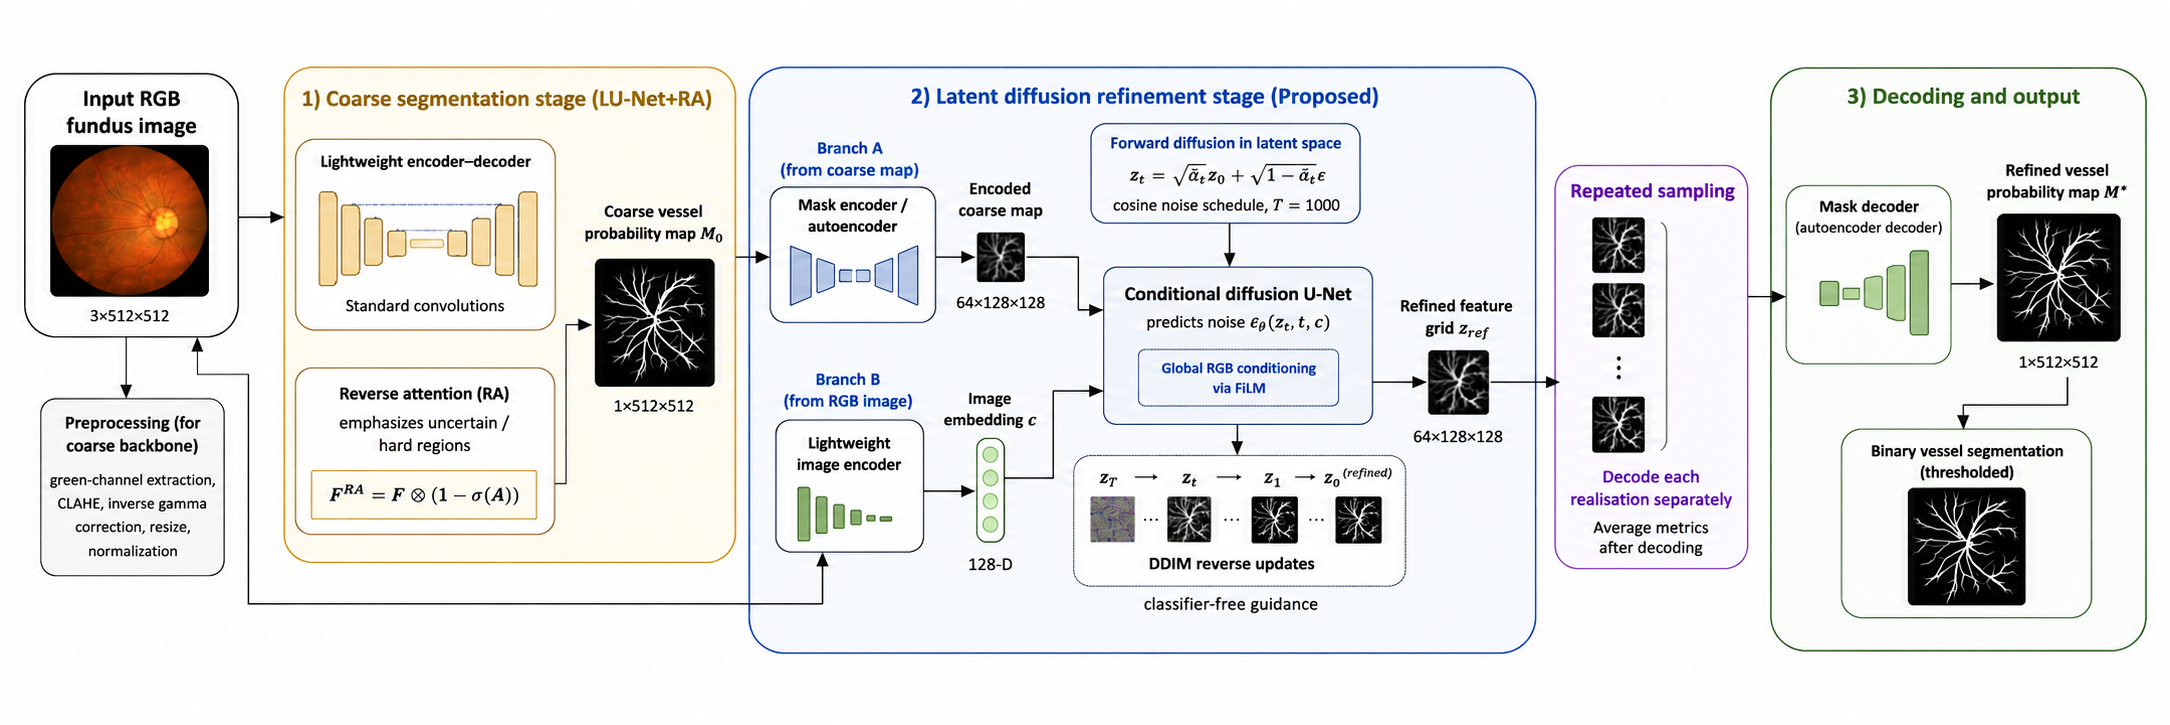
\includegraphics[width=0.98\linewidth]{realdata/flowchart_corrected_2026-10-15_14-14-14.png}}%
    {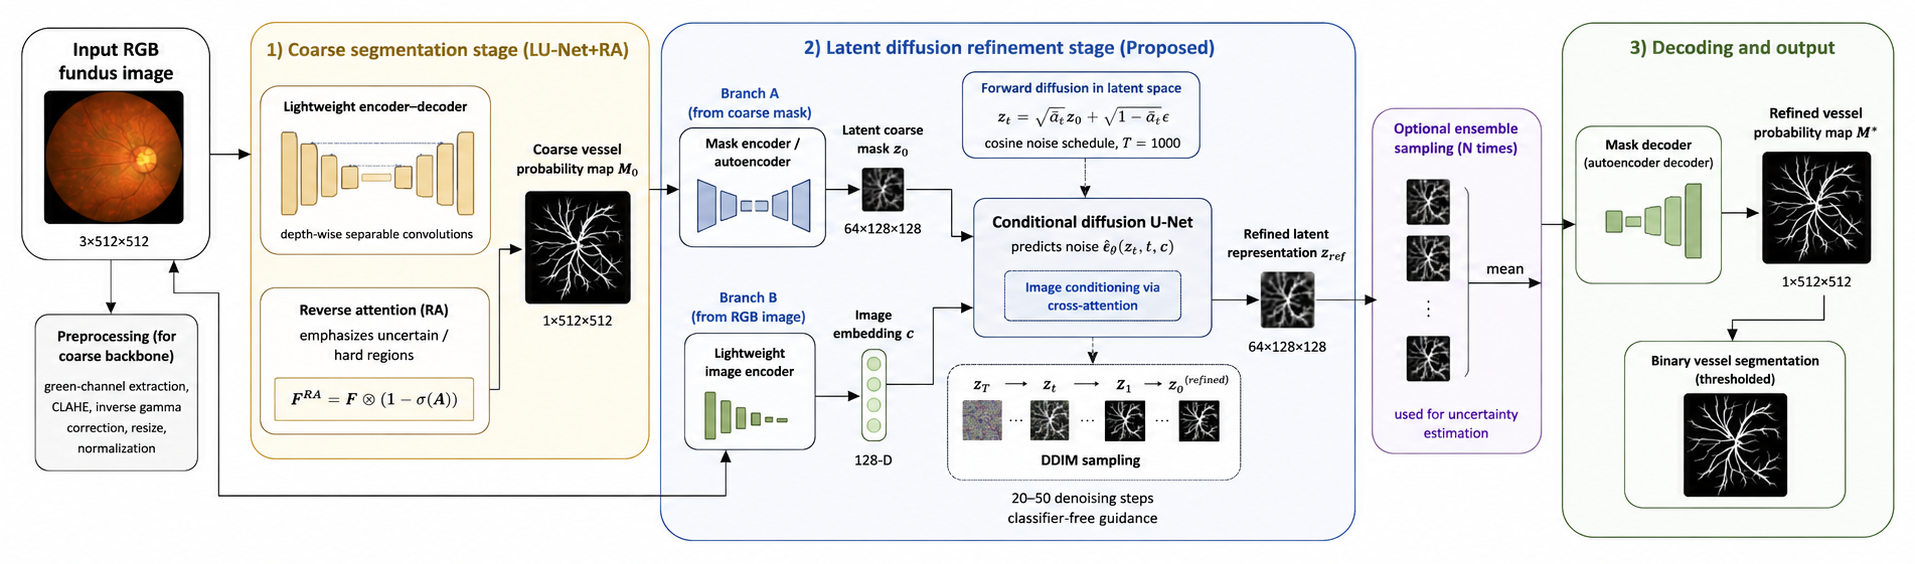
\includegraphics[width=0.98\linewidth]{realdata/flowchart260801-2.png}}
  \caption{Workflow of the proposed two-stage framework. Stage~1 applies vessel-enhancement preprocessing and LU-Net with reverse attention to produce the coarse vessel mask $\mathbf{M}_0$. In Stage~2, the frozen mask encoder maps $\mathbf{M}_0$ to a spatially downsampled \rev{multi-channel} grid, which is noised and refined by the conditional diffusion U-Net using deterministic DDIM \rev{updates}. A separate RGB image encoder supplies the 128-dimensional conditioning vector\rev{, which modulates the denoiser through feature-wise linear modulation (FiLM)}. The frozen mask decoder produces the refined vessel-probability map $\mathbf{M}^{*}$. \rev{When several sampling seeds are evaluated, each realisation is decoded separately and metrics are averaged after decoding.}}
  \label{fig:flowchart_architecture}
\end{figure}

The remainder of this paper is organised as follows. Section~\ref{sec:related} reviews prior work on vessel segmentation and diffusion-based refinement. Section~\ref{sec:methods} describes the coarse predictor and proposed refinement method. Section~\ref{sec:experiments_results} presents the experimental protocol, segmentation results, and qualitative analyses. Sections~\ref{sec:discussion} and~\ref{sec:conclusion} discuss the evidence, limitations, and conclusions.
%%%%%%%%%%%%%%%%%%%%%%%%%%%%%%%%%%%%%%%%%%


%%%%%%%%%%%%%%%%%%%%%%%%%%%%%%%%%%%%%%%%%%

\section{Related Work}
\label{sec:related}
\seclabel{related}

\subsection{Retinal Vessel Segmentation}

Early retinal vessel segmentation methods relied on hand-crafted features, such as Gabor filters and matched filtering, combined with thresholding or classical classifiers~\cite{Soares2006, Mendonca2006}. While effective in controlled settings, these approaches lack robustness to variations in illumination and vessel appearance.

With the advent of deep learning, convolutional neural networks (CNNs), particularly U-Net~\cite{Ronneberger2015}, became the dominant paradigm for biomedical image segmentation, achieving strong performance on benchmark datasets such as DRIVE~\cite{Staal2004}. Subsequent work has focused on improving architectural design, including nested structures (UNet++~\cite{Zhou2018UNetpp}), attention mechanisms~\cite{Oktay2018AttUNet, Schlemper2019AG}, and recurrent or residual connections~\cite{Alom2018R2UNet}, as well as incorporating vessel-specific priors such as connectivity constraints and boundary information~\cite{Fu2016DeepVessel, Liskowski2016, Shin2019Connectivity}.

More recently, lightweight architectures such as LU-Net+RA~\cite{Hernandez2025} have aimed to balance accuracy and efficiency by leveraging depth-wise separable convolutions and reverse attention. Thin-vessel recovery and structural continuity remain relevant evaluation targets, particularly in low-contrast regions. These targets motivate testing whether a separate refinement strategy changes coarse predictions beneficially under a controlled protocol.

\subsection{Diffusion Models}

Diffusion models learn to reverse a progressive noise process~\cite{Ho2020}. DDIM permits deterministic transitions along a reduced timestep sequence~\cite{Song2021}, while latent diffusion performs these updates in an autoencoder representation~\cite{Rombach2022}.

Diffusion models have also been investigated for medical-image segmentation. Wolleb et al.~\cite{Wolleb2022} generated implicit segmentation ensembles, while SegDiff and MedSegDiff adapted conditional diffusion to general and medical segmentation tasks~\cite{SegDiff,MedSegDiff}. Pre-segmentation diffusion sampling starts the reverse process from a noised preliminary mask rather than pure Gaussian noise~\cite{PDDiffusion}, which is conceptually close to the initialisation used here. A broader survey is provided by Kazerouni et al.~\cite{Kazerouni2023}.

Recent work is more directly related to coarse-to-fine refinement. HiDiffSeg combines a coarse vessel estimate, vessel skeleton, and fundus-image guidance in a hierarchical diffusion model for retinal vessel segmentation~\cite{HiDiffSeg}. RefineCatDiff uses a coarse probability map as prior knowledge in a categorical diffusion process for medical-image segmentation~\cite{RefineCatDiff}. Li et al.~\cite{DiffusionFMD} instead introduce a plug-and-play diffusion denoising module for end-to-end feature-map refinement. The present method differs in four respects: it applies continuous Gaussian diffusion to the encoded LU-Net+RA probability map; freezes a mask autoencoder during refinement training; conditions the denoiser with a global RGB embedding; and adds \rev{527,233} parameters as a post-processing stage. These distinctions define the architectural contribution, but they do not establish performance superiority because no controlled comparison with these methods is available. \rev{We did not reproduce these three methods under our protocol: they diffuse different quantities (skeleton-guided hierarchical maps, categorical labels and intermediate feature maps), so each would need a separate implementation and tuning. Because our refiner does not improve its own coarse input (Section~\ref{sec:quantitative}), we compare it instead with two deterministic learned refiners (Sections~\ref{sec:ablations} and~\ref{sec:spatial}).}

Unlike formulations that diffuse an encoded ground-truth target, the proposed training process adds noise to the encoded coarse mask and uses a decoded Dice term to encourage agreement with the reference mask. This choice makes the method a Dice-regularised denoiser of the coarse prediction rather than a conventional target-diffusion model. \rev{Section~\ref{sec:ablations} reports a deterministic learned-refiner control and a target-diffusion ablation that isolate the contribution of the diffusion formulation.}\secend{related}

\subsection{Attention Mechanisms in Medical Imaging}

Attention mechanisms are widely used in medical imaging to enhance feature representation by focusing on relevant regions. Channel and spatial attention modules, such as SE-Net~\cite{Hu2018} and CBAM~\cite{Woo2018}, improve performance by reweighting feature responses. In contrast, reverse attention~\cite{Hernandez2025} explicitly emphasises regions that are likely to be misclassified, enabling the model to focus on difficult structures.


%%%%===========================================================================================================================================
\section{Methods}
\label{sec:methods}

\subsection{Problem Formulation}
\label{sec:problem}

Retinal vessel segmentation is formulated as a dense prediction task in which each pixel of a fundus image is classified as vessel or background. Let $\mathbf{I}\in\mathbb{R}^{3\times512\times512}$ denote an RGB fundus image, and let $\mathbf{M}_{gt}\in\{0,1\}^{1\times512\times512}$ denote the corresponding ground-truth mask. The objective is to learn a mapping $\mathcal{F}:\mathbf{I}\mapsto \mathbf{M}^*$, where $\mathbf{M}^*\in[0,1]^{1\times512\times512}$ is the predicted vessel probability map (thresholded to obtain a binary mask during evaluation).

Instead of a single-stage prediction, we adopt a coarse-to-fine framework. A lightweight segmentation model first produces a coarse estimate $\mathbf{M}_0\in[0,1]^{1\times512\times512}$, which captures the main vessel structure but may contain discontinuities, missing thin vessels, and blurred boundaries.

To refine this estimate, $\mathbf{M}_0$ is mapped to a \rev{spatially downsampled multi-channel} representation $\mathbf{z}_c=\mathrm{Encode}(\mathbf{M}_0)$, where $\mathrm{Encode}(\cdot)$ denotes a mask encoder and $\mathbf{z}_c\in\mathbb{R}^{C\times H\times W}$ is a spatially downsampled learned grid. A conditional diffusion model $\mathrm{Refine}_{\theta}(\cdot)$ then updates $\mathbf{z}_c$ iteratively while conditioning on the input image $\mathbf{I}$. The refined \rev{grid} is mapped back to pixel space using a decoder $\mathrm{Decode}(\cdot)$, yielding:
\begin{equation}
\mathbf{M}^* = \mathrm{Decode}\big(\mathrm{Refine}_{\theta}(\mathbf{z}_c, \mathbf{I})\big).
\end{equation}

This formulation separates coarse prediction from iterative refinement and provides a tunable additional-computation stage.

\subsection{Baseline: Lightweight U-Net with Reverse Attention}

For coarse segmentation, we use LU-Net+RA~\cite{Hernandez2025}, a lightweight encoder--decoder\rev{; the released one-channel LNet\_RA implementation used here employs standard convolutions and reduced channel widths}. Its key component is reverse attention (RA), which emphasises uncertain regions. Given a feature map $\mathbf{F}$ and attention logits $\mathbf{A}$, the RA output is:
\begin{equation}
\mathbf{F}^{\text{RA}} = \mathbf{F}\otimes \left(1-\sigma(\mathbf{A})\right),
\end{equation}
where $\sigma(\cdot)$ is the sigmoid function and $\otimes$ denotes element-wise multiplication. Here, $\sigma(\mathbf{A})$ highlights predicted vessel regions, while its complement focuses the model on hard or misclassified areas. The resulting reverse-attention-modulated features are decoded to produce the coarse prediction $\mathbf{M}_0$ used by the diffusion refinement stage.

Importantly, this RA mechanism is used only within the LU-Net+RA backbone. The diffusion refiner itself does not receive a separate RA map tensor as an additional input. Instead, the diffusion stage is conditioned on the \rev{encoded coarse mask} $\mathbf{z}_c=\mathrm{Encode}(\mathbf{M}_0)$ and the image embedding $\mathbf{c}=\mathrm{ImageEncoder}(\mathbf{I}_{RGB})$. In other words, reverse-attention guidance is implemented implicitly via the RA-enhanced coarse prediction $\mathbf{M}_0$, rather than as an explicit extra conditioning channel in the diffusion U-Net.

\subsection{Proposed Conditional Diffusion Refiner}
\label{sec:refiner}
\seclabel{refiner}

To refine the coarse segmentation, we operate on a learned multi-channel \rev{grid} with lower spatial resolution than the input mask. The proposed refinement framework consists of a mask autoencoder, an image encoder for conditioning, and a conditional diffusion model defined in this learned representation space.
\begin{table}[htbp]\revbegin{}
\centering
\caption{Component interfaces and parameter counts of the refinement module. Counts include frozen components. The executable configuration, used in all experiments, has a time-conditioning MLP; the archived implementation has a separate image-conditioning MLP.}
\label{tab:architecture_params}
\small
\begin{tabularx}{\textwidth}{@{}p{0.22\textwidth}Xrr@{}}
\toprule
Component & Interface and role & Executable & Archived \\
\midrule
Mask autoencoder & $1\times512\times512$ mask $\rightarrow 64\times128\times128$ grid $\rightarrow 1\times512\times512$ probability map & 121,409 & 121,409 \\
Image encoder & $3\times512\times512$ RGB image $\rightarrow$ 128-dimensional global embedding & 27,712 & 27,712 \\
Diffusion U-Net with FiLM projections & Noisy grid, timestep and condition $\rightarrow$ predicted noise & 353,280 & 353,280 \\
Conditioning MLP & Time conditioning (executable) or image conditioning (archived) & 24,832 & 33,024 \\
\midrule
Full refinement module & Coarse probability map and RGB image $\rightarrow$ refined vessel-probability map & \textbf{527,233} & \textbf{535,425} \\
\bottomrule
\end{tabularx}
\revend{}\end{table}
\begin{table}[htbp]\revbegin{}
\centering
\caption{Parameter budgets of LU-Net+RA and the complete two-stage systems. The backbone is frozen during refinement training.}
\label{tab:complete_parameter_counts}
\small
\begin{tabular}{lrrrr}
\toprule
Configuration & Backbone & Added refiner & Complete system & Updated in refinement \\
\midrule
LU-Net+RA & 1,946,961 & 0 & 1,946,961 & 0 \\
Executable refiner & 1,946,961 & 527,233 & 2,474,194 & 405,824 \\
Archived refiner & 1,946,961 & 535,425 & 2,482,386 & 414,016 \\
\bottomrule
\end{tabular}
\revend{}\end{table}
\revbegin{}Parameters are counted as unique registered weights and biases, including frozen modules and excluding buffers and optimizer states. Under this convention the released LU-Net+RA has 1,946,961 parameters; its 3,028 buffer elements are excluded. An earlier subtotal of 502,401 refinement parameters covered the mask autoencoder, image encoder and diffusion U-Net but omitted the archived implementation's separate 33,024-parameter conditioning MLP; including it gives 535,425 parameters, 27.50\% of the backbone. The executable configuration used in all experiments has a 24,832-parameter time-conditioning MLP instead, giving 527,233 refinement parameters, 27.08\% of the backbone (Tables~\ref{tab:architecture_params} and~\ref{tab:complete_parameter_counts}). These counts describe storage and training budgets; sequential sampling adds inference cost, which Section~\ref{sec:latency} measures.\secend{refiner}\revend{}

\subsubsection{Mask Autoencoder}
\label{sec:autoencoder}
\seclabel{autoencoder}

We use a lightweight convolutional autoencoder that maps a vessel mask $\mathbf{M}\in\mathbb{R}^{1\times512\times512}$ to a \rev{multi-channel} grid $\mathbf{z}\in\mathbb{R}^{64\times128\times128}$, corresponding to a $4\times$ reduction along each spatial dimension. The input mask contains $1\times512\times512=262{,}144$ scalar values, whereas the multi-channel grid contains $64\times128\times128=1{,}048{,}576$ values. It is therefore spatially downsampled but not compressed in scalar count. The architecture is:
\begin{itemize}
  \item Encoder: Conv($1\rightarrow32$, $3\times3$, stride 2, padding 1) + ReLU $\rightarrow$ Conv($32\rightarrow64$, $3\times3$, stride 2, padding 1) + ReLU $\rightarrow$ Conv($64\rightarrow64$, $1\times1$, stride 1).
  \item Decoder: two $4\times4$ transposed convolutions ($64\rightarrow64$ and $64\rightarrow32$; stride 2, padding 1), each followed by ReLU, then a $1\times1$ convolution ($32\rightarrow1$) and sigmoid activation.
\end{itemize}

Therefore, the spatial path is $512\times512\rightarrow256\times256\rightarrow128\times128$ in the encoder and $128\times128\rightarrow256\times256\rightarrow512\times512$ in the decoder, while channel progression is $1\rightarrow32\rightarrow64\rightarrow64$ (encoder) and $64\rightarrow64\rightarrow32\rightarrow1$ (decoder). The autoencoder has approximately $0.121$M trainable parameters in total (about $22{,}976$ in the encoder and $98{,}433$ in the decoder).

For an input ground-truth mask $\mathbf{M}_{gt}$, the autoencoder reconstruction is
\begin{equation}
\tilde{\mathbf{M}}=D_m\!\left(E_m(\mathbf{M}_{gt})\right).
\end{equation}
The reconstruction term is the mean squared error over the $N=512\times512$ pixels,
\begin{equation}
\mathcal{L}_{\text{MSE}}(\tilde{\mathbf{M}},\mathbf{M}_{gt})=
\frac{1}{N}\sum_{p=1}^{N}
\left(\tilde{M}_{p}-M_{gt,p}\right)^2.
\end{equation}
For any predicted probability map $\mathbf{P}$ and binary target $\mathbf{G}$, we use the soft Dice loss
\begin{equation}
\mathcal{L}_{\text{Dice}}(\mathbf{P},\mathbf{G})=
1-\frac{2\sum_{p=1}^{N}P_pG_p}
{\sum_{p=1}^{N}P_p+\sum_{p=1}^{N}G_p}.
\end{equation}
Accordingly, the autoencoder objective is
\begin{equation}
\mathcal{L}_{\text{AE}} =
\mathcal{L}_{\text{MSE}}(\tilde{\mathbf{M}},\mathbf{M}_{gt})+
\mathcal{L}_{\text{Dice}}(\tilde{\mathbf{M}},\mathbf{M}_{gt}).
\end{equation}
All sums are evaluated over the complete resized mask\rev{ and pooled over the images in a minibatch; the implemented Dice adds $\varepsilon=10^{-6}$ to its numerator and denominator}. \rev{For CHASE-DB1 and HRF, the} autoencoder is pretrained on ground-truth masks only, without additional mask augmentation\rev{, for 50 epochs with AdamW (learning rate $10^{-4}$, weight decay $10^{-3}$), keeping the checkpoint with the highest validation soft Dice. For DRIVE, it is trained for 200 epochs with AdamW (learning rate $10^{-3}$, weight decay $10^{-3}$, cosine schedule) on equal batches of in-sample coarse maps and reference masks, reconstructing each input, and the checkpoint with the lowest validation coarse-map reconstruction error is kept}. After pretraining, its parameters are frozen and used to encode $\mathbf{M}_0$. The distribution shift between binary training masks and soft coarse probability maps is analysed as a limitation in Section~\ref{sec:limitations}.\secend{autoencoder}

\subsubsection{Image Conditioning}

To incorporate global contextual information, the diffusion refinement stage uses a custom lightweight CNN image encoder (not ResNet/MobileNet) fed by the resized and normalised RGB fundus image. Specifically, the encoder receives $\mathbf{I}_{RGB}\in\mathbb{R}^{3\times512\times512}$ and maps it to a compact feature vector $\mathbf{c}\in\mathbb{R}^{128}$:
\begin{equation}
\mathbf{c}=\mathrm{ImageEncoder}(\mathbf{I}_{RGB}).
\end{equation}

Its layer stack is:
\begin{itemize}
  \item Conv($3\rightarrow32$, $3\times3$, stride 2, padding 1) + ReLU,
  \item Conv($32\rightarrow64$, $3\times3$, stride 2, padding 1) + ReLU,
  \item Adaptive average pooling to $1\times1$,
  \item Flatten,
  \item Linear($64\rightarrow128$) to produce the final embedding $\mathbf{c}$.
\end{itemize}

Thus, the feature map is downsampled as $512\times512\rightarrow256\times256\rightarrow128\times128\rightarrow1\times1$, then projected to a 128-dimensional conditioning vector. This image encoder has approximately $0.028$M trainable parameters ($27{,}712$ parameters) and is trained from scratch during diffusion-refiner training (no external pretrained weights are used).

This RGB conditioning branch is separate from the preprocessing used by the coarse LU-Net+RA segmentation backbone. The backbone follows the vessel-enhancement preprocessing pipeline, including green-channel extraction and contrast enhancement, to produce the coarse vessel probability map $\mathbf{M}_0$. In contrast, the diffusion image encoder is not given a green-channel-only image or a CLAHE-enhanced single-channel input; it receives the three-channel RGB fundus image after resizing and normalisation. This design allows the refiner to exploit colour and illumination cues while the diffusion process operates on the encoded coarse mask.
\subsubsection{Diffusion on the Encoded Grid}
\label{sec:diffusion_process}
\seclabel{diffusion_process}

The refinement is formulated as a diffusion process in the encoded \rev{representation}. Starting from the encoded coarse mask $\mathbf{z}_c=\mathrm{Encode}(\mathbf{M}_0)$, noise is progressively added according to a cosine schedule~\cite{Nichol2021}:
\begin{equation}
\rev{a_t}=\frac{\cos^2\!\left(\frac{t/T+0.008}{1.008}\cdot\frac{\pi}{2}\right)}{\cos^2\!\left(\frac{0.008}{1.008}\cdot\frac{\pi}{2}\right)},
\end{equation}
where $t\in\{0,\dots,T\}$ denotes the diffusion step \rev{and $T=1000$. The implementation derives per-step rates $\beta_k=\min(1-a_{k+1}/a_k,\,0.999)$ and stores the cumulative signal-retention products $\bar{\alpha}_k=\prod_{j=0}^{k}(1-\beta_j)$ for the zero-based indices $k=0,\ldots,999$, so the stored $\bar{\alpha}_0$ is slightly below one. Training timesteps are sampled uniformly from $\{0,\ldots,999\}$, and inference uses 50 DDIM updates (Section~\ref{sec:ddim_sampling}).} The forward process generates noisy \rev{encoded} variables:
\begin{equation}
\mathbf{z}_t=\sqrt{\bar{\alpha}_t}\mathbf{z}_c+\sqrt{1-\bar{\alpha}_t}\,\boldsymbol{\epsilon}, 
\quad \boldsymbol{\epsilon}\sim\mathcal{N}(0,\mathbf{I}),
\end{equation}
where $\boldsymbol{\epsilon}$ is Gaussian noise. The clean encoder output is denoted by $\mathbf{z}_c$ to distinguish it from the noisy variable at stored schedule index zero.

A conditional diffusion U-Net is then trained to reverse this process by predicting the noise component $\hat{\boldsymbol{\epsilon}}_\theta(\mathbf{z}_t,t,\mathbf{c})$, conditioned on both the noisy \rev{encoded} tensor $\mathbf{z}_t$ and the image embedding $\mathbf{c}$.


\subsubsection{Conditioning Injection \rev{and Denoiser Layers}}
\label{sec:conditioning}
\seclabel{conditioning}

\rev{In the executable configuration, a $64\rightarrow128\rightarrow128$ MLP with SiLU projects the sinusoidal timestep embedding and adds it to the 128-dimensional image embedding $\mathbf{c}$. In each residual block of the diffusion U-Net, a $128\rightarrow128$ linear projection of this combined vector supplies 64 scales and 64 shifts for feature-wise linear modulation (FiLM). Each residual block applies GroupNorm with eight groups, SiLU, a convolution, FiLM, a second convolution and SiLU, and then adds the block input; Table~\ref{tab:denoiser_layers} lists the layers.} This feature-wise conditioning supplies global fundus context throughout denoising without introducing a separate spatial cross-attention map. Reverse attention remains confined to the LU-Net+RA backbone that produces the coarse mask $\mathbf{M}_0$; no separate RA tensor is injected into the diffusion U-Net. \rev{Residual connections are internal to the blocks; there is no additional encoder--decoder concatenation skip. The output predicts noise.}\secend{conditioning}

\begin{table}[htbp]\revbegin{}
\centering
\caption{Layers of the diffusion U-Net (denoiser) in the executable configuration. The encoded input has 64 channels.}
\label{tab:denoiser_layers}
\small
\begin{tabular}{llll}
\toprule
Layer & Channels & Kernel / stride / padding & Spatial size \\
\midrule
Input convolution & $64\rightarrow64$ & 3 / 1 / 1 & $128\times128$ \\
Residual FiLM block & $64\rightarrow64$ & Two 3 / 1 / 1 convolutions & $128\times128$ \\
Down convolution & $64\rightarrow64$ & 4 / 2 / 1 & $64\times64$ \\
Residual FiLM block & $64\rightarrow64$ & Two 3 / 1 / 1 convolutions & $64\times64$ \\
Transpose convolution & $64\rightarrow64$ & 4 / 2 / 1 & $128\times128$ \\
Output convolution & $64\rightarrow64$ & 1 / 1 / 0 & $128\times128$ \\
\bottomrule
\end{tabular}
\revend{}\end{table}

\subsubsection{Training Objective}
\label{sec:objective}
\seclabel{objective}

The model is trained to predict the noise added during the forward diffusion process while incorporating segmentation-aware constraints. Let $N_z$ be the number of elements in \rev{an encoded} tensor. The mean DDPM noise-prediction loss is
\begin{equation}
\mathcal{L}_{\text{DDPM}}=
\mathbb{E}_{\mathbf{z}_c,t,\boldsymbol{\epsilon}}\left[
\frac{1}{N_z}\left\|
\hat{\boldsymbol{\epsilon}}_\theta(\mathbf{z}_t,t,\mathbf{c})-
\boldsymbol{\epsilon}
\right\|_2^2
\right],
\end{equation}
with $\boldsymbol{\epsilon}\sim\mathcal{N}(0,\mathbf{I})$ denoting Gaussian noise and $\mathbf{z}_t$ the noisy \rev{encoded} tensor obtained from $\mathbf{z}_c$ at timestep $t$.
The noise prediction is then used to estimate the clean \rev{encoded} tensor corresponding to the sampled timestep:
\begin{equation}
\hat{\mathbf{z}}_c^{(t)}=
\frac{\mathbf{z}_t-
\sqrt{1-\bar{\alpha}_t}\,
\hat{\boldsymbol{\epsilon}}_\theta(\mathbf{z}_t,t,\mathbf{c})}
{\sqrt{\bar{\alpha}_t}}.
\end{equation}
Because the pretrained mask decoder is frozen and includes its output sigmoid, the associated vessel-probability map is
\begin{equation}
\hat{\mathbf{M}}_t=D_m\!\left(\hat{\mathbf{z}}_c^{(t)}\right).
\end{equation}
The segmentation-aware term is therefore $\mathcal{L}_{\text{Dice}}(\hat{\mathbf{M}}_t,\mathbf{M}_{gt})$, using the pixel-space definition given above, and the complete diffusion-refiner objective is
\begin{equation}
\mathcal{L}=
\mathcal{L}_{\text{DDPM}}+
\lambda_{\text{dice}}
\mathcal{L}_{\text{Dice}}(\hat{\mathbf{M}}_t,\mathbf{M}_{gt}).
\end{equation}
In the implementation evaluated here, $\lambda_{\text{dice}}=0.5$; no separate Sobel edge-loss term is applied. \rev{This weight was fixed in advance and not tuned.}

This objective is Dice-regularised denoising of the encoded coarse mask. The DDPM term is defined with respect to Gaussian noise added to $E_m(\mathbf{M}_0)$ and therefore favours recovery of the coarse \rev{encoded} grid, whereas the decoded Dice term encourages agreement with the ground-truth vessel mask. The method is not formulated as unconditional generation of $E_m(\mathbf{M}_{gt})$. This distinction is important when comparing it with formulations that diffuse the ground-truth target and provide the coarse mask as a separate condition.

The models are trained in two stages. The mask autoencoder is pretrained \rev{as described in Section~\ref{sec:autoencoder}}. Its weights are then frozen, and the diffusion refiner is trained for 100 epochs using AdamW at $1\times10^{-4}$ with cosine annealing over the full training schedule\rev{, weight decay $10^{-3}$, batch size four and gradient clipping at one; the predefined final epoch-100 checkpoint is evaluated}. During diffusion training, only the image encoder, conditioning multilayer perceptron (MLP), and diffusion U-Net are updated. A classifier-free-guidance conditioning dropout of 10\% is applied during training. No additional image or mask augmentation is used. Images and masks are resized to $512\times512$, and LU-Net+RA probability maps are loaded as the coarse conditions. No explicit field-of-view loss mask or crop is applied during refiner training.\secend{objective}

\subsubsection{DDIM Sampling}
\label{sec:ddim_sampling}
\seclabel{ddim_sampling}

For inference, we employ DDIM sampling~\cite{Song2021} to generate a refined \rev{encoded} representation from the initial code $\mathbf{z}_c=\mathrm{Encode}(\mathbf{M}_0)$. Instead of starting from pure noise, the sampling process is initialised from a noisy version of $\mathbf{z}_c$, preserving an explicit connection to the coarse prediction throughout the refinement trajectory.

\begin{table}[htbp]
\caption{\rev{Refinement} sampling procedure \rev{of the executable configuration}.}
\label{alg:latent_refinement}
\centering
\begin{minipage}{0.96\textwidth}
\small
\revbegin{}\textbf{Inputs:} coarse mask $\mathbf{M}_0$; RGB image $\mathbf{I}_{RGB}$; encoders $E_m,E_I$; decoder $D_m$; noise network $\boldsymbol{\epsilon}_\theta$; stored schedule $\{\bar{\alpha}_k\}_{k=0}^{999}$; start index $t_s=99$; number of DDIM updates $S$; guidance scale $s=1.5$.\par
\begin{enumerate}[leftmargin=2em,itemsep=2pt,topsep=4pt]
  \item Encode $\mathbf{z}_c=E_m(\mathbf{M}_0)$ and $\mathbf{c}=E_I(\mathbf{I}_{RGB})$; set the null condition $\mathbf{c}_{\emptyset}=\mathbf{0}$.
  \item Set $t_i=\lfloor t_s(1-i/(S-1))\rfloor$ for $i=0,\ldots,S-1$, so $t_0=t_s$ and $t_{S-1}=0$.
  \item Draw $\boldsymbol{\epsilon}\sim\mathcal{N}(0,\mathbf{I})$ and initialise $\mathbf{z}=\sqrt{\bar{\alpha}_{t_0}}\mathbf{z}_c+\sqrt{1-\bar{\alpha}_{t_0}}\boldsymbol{\epsilon}$.
  \item For $i=0,\ldots,S-1$, evaluate $\boldsymbol{\epsilon}_{c}=\boldsymbol{\epsilon}_\theta(\mathbf{z},t_i,\mathbf{c})$ and $\boldsymbol{\epsilon}_{u}=\boldsymbol{\epsilon}_\theta(\mathbf{z},t_i,\mathbf{c}_{\emptyset})$, and form $\hat{\boldsymbol{\epsilon}}=\boldsymbol{\epsilon}_{u}+s(\boldsymbol{\epsilon}_{c}-\boldsymbol{\epsilon}_{u})$.
  \item Estimate $\hat{\mathbf{z}}_c=(\mathbf{z}-\sqrt{1-\bar{\alpha}_{t_i}}\hat{\boldsymbol{\epsilon}})/\sqrt{\bar{\alpha}_{t_i}}$; set $B=\bar{\alpha}_{t_{i+1}}$ if $i<S-1$ and $B=1$ otherwise; update $\mathbf{z}\leftarrow\sqrt{B}\hat{\mathbf{z}}_c+\sqrt{1-B}\hat{\boldsymbol{\epsilon}}$.
  \item Return $\mathbf{M}^*=D_m(\mathbf{z})$.
\end{enumerate}\revend{}
\end{minipage}
\end{table}

The starting timestep $t_s$ controls refinement strength: a larger value adds more noise to the encoded coarse mask and permits a stronger correction, whereas a smaller value preserves more of the LU-Net+RA prediction. \rev{Coarse-initialised diffusion uses $t_s=99$. The target-diffusion Gaussian-start ablation instead starts from pure Gaussian noise at index 999, and the deterministic encoded-grid control uses no DDIM sampling. The strength $\rho$ of the earlier single-run experiment was not recorded. The $S$ retained indices are spaced by integer truncation between $t_s$ and zero, and the last update projects from index zero to the clean endpoint, so $S$ counts the denoiser-driven updates (DDIM transitions).} At every reverse step, the diffusion U-Net is evaluated with both the image condition and a null condition. Their predictions are combined using classifier-free guidance\rev{ with scale 1.5}, after which the deterministic DDIM update ($\eta_{\mathrm{DDIM}}=0$) maps the current feature tensor to the next timestep. Because the mask decoder already ends with a sigmoid activation, the procedure in Table~\ref{alg:latent_refinement} does not apply a second sigmoid. \rev{Each trained stochastic refiner in the matched repeated-training study is evaluated with five initial-noise seeds; each realisation is decoded separately, and metrics, rather than probability maps, are averaged. The fixed-checkpoint repeated-sampling experiment has a separate protocol (Section~\ref{sec:ddim_count}).} Although each reverse trajectory is deterministic after its initial noise sample is fixed, the complete procedure remains stochastic with respect to that initial sample.\secend{ddim_sampling}

%%%%===========================================================================================================================================
%%%%===========================================================================================================================================

\section{Experiments and Results}
\label{sec:experiments_results}

\subsection{Datasets and Preprocessing}
\label{sec:datasets}
\seclabel{datasets}

We evaluate the refiner on three public retinal vessel datasets: the Child Heart and Health Study in England Database 1 (CHASE-DB1)~\cite{CHASEDB1}, Digital Retinal Images for Vessel Extraction (DRIVE)~\cite{Staal2004}, and High-Resolution Fundus (HRF)~\cite{Odstrcilik2013HRF}. Table~\ref{tab:datasets} reports the released image sizes used by the preprocessing pipeline and the \rev{fitting, validation and test partitions used in the reference and matched encoded-grid experiments}.

\begin{table}[htbp]
\centering
\caption{Dataset composition and partitions \rev{used in all experiments}. Image sizes refer to the released or cropped images used by the pipeline, not necessarily the acquisition resolution. \rev{Partitions use split seed 42 and are fixed across training seeds.}}
\label{tab:datasets}
\small
\begin{tabularx}{\textwidth}{@{}l c c X c@{}}
\toprule
Dataset & Images & Released Image Size & \rev{Fitting / validation / test} & Test $n$ \\
\midrule
CHASE-DB1 & 28 & $999\times960$ & \rev{16 / 4 / 8} & 8 \\
DRIVE & 40 & $565\times584$ & \rev{16 / 4 / 20} & 20 \\
HRF & 45 & $3504\times2336$ & \rev{27 / 6 / 12} & 12 \\
\bottomrule
\end{tabularx}
\end{table}

CHASE-DB1 contains images of both eyes from 14 children\rev{; its partitions are grouped by subject (8/2/4 subjects), keeping both eyes of each child together, and first-observer annotations are used for all evaluations}. DRIVE has an official 20-image training set and 20-image test set\rev{; its training pool is split into 16 fitting and four validation images}. HRF contains 15 healthy, 15 diabetic-retinopathy, and 15 glaucomatous images\rev{; its partitions are stratified by group, with 9/2/4 fitting/validation/test images per group. The HRF field-of-view masks are decoded from Supervisely-format annotation files, whose conversion from the original annotations is not documented.}

Two preprocessing streams are used. The LU-Net+RA backbone follows the preprocessing pipeline of Hernandez-Gutierrez et al.~\cite{Hernandez2025}: green-channel extraction, contrast-limited adaptive histogram equalisation (CLAHE), inverse gamma correction, resizing to $512\times512$, and normalisation to $[0,1]$. This stream produces the coarse probability map $\mathbf{M}_0$. The refiner receives $\mathbf{M}_0$, while its image encoder receives the corresponding resized and normalised RGB fundus image. \rev{RGB images and the preprocessed green channel are resized with bilinear interpolation, and binary annotations and FOV masks with nearest-neighbour interpolation, on a square canvas without preserving the native aspect ratio.}\secend{datasets}

\subsection{Training and Implementation Details}
\label{sec:training}
\seclabel{training}

Training is sequential. LU-Net+RA is trained first and then frozen. Its stored probability maps condition the refiner, whose training does not update the backbone. The coarse maps used to train the refiner were generated from images that had also been used to fit LU-Net+RA; they are therefore in-sample rather than out-of-fold predictions. Freezing prevents joint adaptation between the stages, but it does not remove the possible train-test shift between in-sample coarse predictions and predictions for unseen images.

\rev{LU-Net+RA is trained with Dice loss and AdamW (learning rate $10^{-3}$, weight decay $10^{-3}$), batch size four, at most 1000 epochs and early stopping with patience 20, keeping the checkpoint with the highest validation mean image Dice; its training applies aligned rotations (0, 15, 30, 45, 90, 100 and 120 degrees) and independent horizontal and vertical flips with probability 0.5.} The mask autoencoder and reference refiner are trained as described in Section~\ref{sec:refiner}; the refiner uses conditioning dropout \rev{of} 10\% and no additional geometric, image, or mask augmentation\rev{; no test result is used for checkpoint selection. The reference and matched encoded-grid configurations are trained five times, with seeds 42, 123, 2026, 3000 and 3001 and the same fixed partitions; each seed is a separate training run, and refiner optimisation noise and dropout use the training seed plus 98765, identically across matched variants. Each trained refiner is evaluated with five initial-noise seeds (42, 123, 2026, 3000 and 3001). For these repeated-training configurations, FP32 test predictions, annotations, FOV masks and confusion counts are saved, and their metrics are computed from these outputs. The spatial refiner uses its separate augmentation recipe (Section~\ref{sec:spatial}). Section~\ref{sec:ddim_count} instead uses one fixed trained model and twenty initial-noise seeds; its archived score and timing records are retained, but complete repeat-level probability arrays were not retained for fresh mask-level verification.}

\rev{Timing uses one NVIDIA GeForce RTX 4070 Ti SUPER graphics processing unit in evaluation mode, with gradient computation disabled, FP32 and a batch size of 1; Sections~\ref{sec:ddim_count} and~\ref{sec:latency} give the measurement protocols.}\secend{training}

\subsection{Evaluation Protocol and Metrics}
\label{sec:metrics}
\seclabel{metrics}

Vessel pixels are treated as the positive class. Let TP, TN, FP, and FN denote true-positive, true-negative, false-positive, and false-negative pixel counts, respectively. The metrics appearing in the result tables are
\begin{align}
\mathrm{Dice} &= \frac{2\mathrm{TP}}{2\mathrm{TP}+\mathrm{FP}+\mathrm{FN}}, \\
\mathrm{Accuracy} &= \frac{\mathrm{TP}+\mathrm{TN}}
{\mathrm{TP}+\mathrm{TN}+\mathrm{FP}+\mathrm{FN}}, \\
\mathrm{Sensitivity} &= \frac{\mathrm{TP}}{\mathrm{TP}+\mathrm{FN}}, \\
\mathrm{Specificity} &= \frac{\mathrm{TN}}{\mathrm{TN}+\mathrm{FP}}.
\end{align}
\rev{Predictions are binarised at probability 0.5. Metrics are computed per image, over the whole image for CHASE-DB1 and within the field-of-view (FOV) mask for DRIVE and HRF, and then averaged over images rather than pooled over pixels.} Training losses, by contrast, were evaluated over the full resized canvas, with pixels outside the retinal field represented as background.

\revbegin{}For each configuration, we average the five sampling realisations within each image and training seed, then average the test images within each seed. Tables report the mean and sample SD across the five seed means; sampling draws do not create additional patients or training runs. Paired comparisons use the five matched seed means, with two-sided paired $t$ tests and exact Wilcoxon signed-rank tests and Holm correction within each stated family. With five pairs, the smallest attainable two-sided exact signed-rank probability is 0.0625. Percentile intervals come from a crossed bootstrap with 50,000 draws that jointly resamples training seeds and test units, keeping both eyes of each CHASE-DB1 subject together and resampling HRF images within pathology groups.\secend{metrics}\revend{}

\subsection{Quantitative Segmentation Results}
\label{sec:quantitative}
\seclabel{quantitative}

\revbegin{}Table~\ref{tab:segmentation_results} compares the coarse LU-Net+RA predictions with the diffusion refiner (global FiLM conditioning, frozen mask autoencoder, 50 updates) on the same test images: eight CHASE-DB1 images from four subjects, twenty DRIVE images and twelve HRF images. For each training seed, both arms use the same LU-Net+RA checkpoint, annotations, FOV masks, threshold and metric code. Refinement lowered mean Dice on all three datasets, by 0.064 on CHASE-DB1, 0.002 on DRIVE and 0.066 on HRF, so the refiner did not improve its coarse input under this protocol.

\begin{table}[htbp]\revbegin{}
\centering
\caption{Paired coarse LU-Net+RA and global/frozen diffusion-refiner Dice at 50 DDIM updates on the same test images. Means and sample SDs are across five training-seed means after averaging five sampling realisations within each image and run. Differences are refiner minus coarse. The 95\% intervals are exploratory paired crossed-bootstrap percentile intervals, not simultaneous confidence intervals.}
\label{tab:segmentation_results}
\small
\resizebox{\linewidth}{!}{%
\begin{tabular}{lrrr}
\toprule
Dataset & Coarse mean $\pm$ SD & Refiner mean $\pm$ SD & Difference \\
\midrule
CHASE-DB1 & $0.810514\pm0.001806$ & $0.746146\pm0.002622$ & $-0.064368245$ \\
DRIVE & $0.791814\pm0.007557$ & $0.789757\pm0.008286$ & $-0.002057107$ \\
HRF & $0.732121\pm0.003490$ & $0.665726\pm0.006320$ & $-0.066395394$ \\
\bottomrule
\end{tabular}}
\par\medskip
\begin{tabular}{lr}
\toprule
Dataset & Paired crossed-bootstrap 95\% interval \\
\midrule
CHASE-DB1 & $[-0.078706654,-0.050060076]$ \\
DRIVE & $[-0.003024955,-0.001308524]$ \\
HRF & $[-0.074121150,-0.058866677]$ \\
\bottomrule
\end{tabular}
\revend{}\end{table}

An earlier single-run experiment with an archived version of this refiner reported Dice of 0.835 on CHASE-DB1, 0.835 on DRIVE and 0.793 on HRF at 50 updates, with 20-update values of 0.825, 0.795 and 0.762 and CHASE-DB1 values from 0.814 at 10 updates to 0.836 at 100 updates. The checkpoint and per-image predictions of that run are no longer available, and its refinement strength, split identities and several training settings were not recorded. The re-implementation documented in Sections~\ref{sec:methods} and~\ref{sec:datasets}--\ref{sec:metrics}, trained with five seeds, did not reproduce these scores (Table~\ref{tab:segmentation_results}). We therefore no longer report them as results.\secend{quantitative}
\subsubsection{Paired Per-Image Analysis and Uncertainty}
\label{sec:paired_per_image}
\seclabel{paired_per_image}
The comparison uses only the global/frozen reference records underlying Table~\ref{tab:segmentation_results}: 1000 image--training-seed--sampling-seed records at 50 updates, comprising eight CHASE-DB1, twenty DRIVE and twelve HRF images, five training seeds and five sampling seeds. Both arms use the same cases, coarse checkpoints and evaluation protocol; scores from other refiner variants are excluded. Sampling realisations are averaged within each image and training seed. Per-image entries then average the five training-seed means, while dataset means and sample SDs summarise five run means on the fixed test set. The coarse prediction is repeated across sampling labels and is not counted as an additional independent observation.

For each dataset, an exploratory paired crossed bootstrap uses 50,000 replicates and random seed 20261017. Training seeds and test units are sampled independently with replacement, retaining matched coarse and refined observations. Both CHASE-DB1 eyes remain together within each of four subjects; DRIVE uses image resampling; HRF resamples images within healthy, diabetic-retinopathy and glaucoma strata. Sampling realisations are averaged before resampling. The 2.5th and 97.5th percentiles form the 95\% interval. All three intervals for refiner-minus-coarse Dice lie below zero, describing lower mean Dice in this tested configuration. Only four CHASE subjects and five training pairs are available, patient independence is unverified for DRIVE and HRF, and these intervals are exploratory rather than confirmatory or simultaneous. These exploratory intervals are not used as confirmatory hypothesis tests.

\begin{table}[htbp]
\centering
\caption{CHASE-DB1 per-image Dice for the Table~\ref{tab:segmentation_results} global/frozen comparison. Each entry averages five training seeds and five sampling realisations. Differences use unrounded paired values and are refined minus coarse. These are per-image means, not independent training replicates.}
\label{tab:paired_per_image_chase}
\small
\begin{tabular}{lrrr}
\toprule
Image & Coarse Dice & Refined Dice & Difference \\
\midrule
Image\_02L & 0.818734630 & 0.771136464 & $-0.047598166$ \\
Image\_02R & 0.812283518 & 0.751455743 & $-0.060827775$ \\
Image\_05L & 0.838999001 & 0.797081068 & $-0.041917933$ \\
Image\_05R & 0.844530892 & 0.792050546 & $-0.052480346$ \\
Image\_09L & 0.805841453 & 0.731423930 & $-0.074417523$ \\
Image\_09R & 0.796916619 & 0.714857283 & $-0.082059336$ \\
Image\_13L & 0.791873375 & 0.720846888 & $-0.071026487$ \\
Image\_13R & 0.774932693 & 0.690314297 & $-0.084618395$ \\
\bottomrule
\end{tabular}
\end{table}

\begin{table}[htbp]
\centering
\caption{DRIVE per-image Dice for the Table~\ref{tab:segmentation_results} global/frozen comparison. Each entry averages five training seeds and five sampling realisations. Differences use unrounded paired values and are refined minus coarse. These are per-image means, not independent training replicates.}
\label{tab:paired_per_image_drive}
\small
\begin{tabular}{lrrr}
\toprule
Image & Coarse Dice & Refined Dice & Difference \\
\midrule
01\_test & 0.797339317 & 0.794007225 & $-0.003332091$ \\
02\_test & 0.827097574 & 0.825196260 & $-0.001901314$ \\
03\_test & 0.787253664 & 0.786541740 & $-0.000711924$ \\
04\_test & 0.804377016 & 0.803009682 & $-0.001367334$ \\
05\_test & 0.796903799 & 0.795544806 & $-0.001358993$ \\
06\_test & 0.785758622 & 0.784951564 & $-0.000807059$ \\
07\_test & 0.800206530 & 0.798486843 & $-0.001719688$ \\
08\_test & 0.780960260 & 0.780790909 & $-0.000169351$ \\
09\_test & 0.783184112 & 0.781780944 & $-0.001403168$ \\
10\_test & 0.785465793 & 0.783200607 & $-0.002265187$ \\
11\_test & 0.773603814 & 0.770267795 & $-0.003336018$ \\
12\_test & 0.796731264 & 0.794527796 & $-0.002203469$ \\
13\_test & 0.793268994 & 0.791305020 & $-0.001963973$ \\
14\_test & 0.789992603 & 0.787225844 & $-0.002766760$ \\
15\_test & 0.763721378 & 0.760549461 & $-0.003171917$ \\
16\_test & 0.808823898 & 0.806945119 & $-0.001878779$ \\
17\_test & 0.789437261 & 0.788254205 & $-0.001183056$ \\
18\_test & 0.786173247 & 0.783883103 & $-0.002290144$ \\
19\_test & 0.802160850 & 0.796962869 & $-0.005197981$ \\
20\_test & 0.783827712 & 0.781713769 & $-0.002113943$ \\
\bottomrule
\end{tabular}
\end{table}

\begin{table}[htbp]
\centering
\caption{HRF per-image Dice for the Table~\ref{tab:segmentation_results} global/frozen comparison. Each entry averages five training seeds and five sampling realisations. Differences use unrounded paired values and are refined minus coarse. These are per-image means, not independent training replicates.}
\label{tab:paired_per_image_hrf}
\small
\begin{tabular}{lrrr}
\toprule
Image & Coarse Dice & Refined Dice & Difference \\
\midrule
01\_g & 0.710632836 & 0.652227842 & $-0.058404994$ \\
02\_h & 0.798816139 & 0.732067972 & $-0.066748166$ \\
04\_g & 0.741554084 & 0.679006689 & $-0.062547395$ \\
07\_dr & 0.733975667 & 0.665890830 & $-0.068084837$ \\
09\_h & 0.750261145 & 0.696942602 & $-0.053318542$ \\
10\_dr & 0.729617456 & 0.653905035 & $-0.075712421$ \\
12\_dr & 0.697127260 & 0.636196628 & $-0.060930632$ \\
13\_g & 0.703959510 & 0.629480025 & $-0.074479486$ \\
13\_h & 0.775788553 & 0.708332717 & $-0.067455836$ \\
14\_g & 0.701151591 & 0.632459952 & $-0.068691639$ \\
14\_h & 0.762417806 & 0.686256277 & $-0.076161529$ \\
15\_dr & 0.680150127 & 0.615940874 & $-0.064209253$ \\
\bottomrule
\end{tabular}
\end{table}

\FloatBarrier
\subsubsection{Matched Out-of-Fold Coarse-Map Training}
\label{sec:oof}
\seclabel{oof}
The separate matched OOF experiment uses four subject-grouped CHASE-DB1 folds, four DRIVE image folds and three pathology-stratified HRF folds, with fold membership fixed using seed 20261009 across the five training seeds. Each fold predictor is fitted without its held-out images and selected using the separate original validation partition. Held-out fold images and test images are not used for checkpoint selection. Both eyes of each CHASE subject remain together. The experiment comprises 55 fold-baseline fits and 15 OOF-refiner fits. The in-sample arm is the global/frozen reference in Table~\ref{tab:segmentation_results}. Both arms share the coarse predictor for the fixed test images, frozen initial mask autoencoder, refiner initialisation, optimisation settings and matched sampling seeds.

The matched OOF evaluation averages the sampling realisations before comparison. Five sampling realisations were averaged within each image and training seed, yielding 200 paired image--training-seed records. OOF crossed-bootstrap intervals use 50,000 replicates and seed 20261015, retaining both eyes within CHASE subjects and HRF pathology strata. The OOF-minus-in-sample tests use five matched training-seed means, with Holm correction across the three datasets separately for paired $t$ and exact signed-rank tests. These intervals describe the OOF-minus-in-sample contrast; they are distinct from the coarse-versus-refiner intervals in Table~\ref{tab:segmentation_results}.

\begin{table}[htbp]
\centering
\caption{Matched OOF versus in-sample refinement at 50 DDIM updates. The in-sample means and SDs match the global/frozen reference in Table~\ref{tab:segmentation_results}. Differences are OOF minus in-sample. Intervals are exploratory crossed-bootstrap intervals; probabilities are Holm-corrected paired training-seed tests, with correction across three datasets separately for each test family.}
\label{tab:matched_oof_existing}
\small
\resizebox{\linewidth}{!}{%
\begin{tabular}{lrrr}
\toprule
Dataset & In-sample mean $\pm$ SD & OOF mean $\pm$ SD & Difference \\
\midrule
CHASE-DB1 & $0.746145777\pm0.002622483$ & $0.745915967\pm0.002732575$ & $-0.000229810$ \\
DRIVE & $0.789757278\pm0.008286356$ & $0.789614005\pm0.008314270$ & $-0.000143273$ \\
HRF & $0.665725620\pm0.006319839$ & $0.665522152\pm0.006144710$ & $-0.000203468$ \\
\bottomrule
\end{tabular}}
\par\medskip
\begin{tabular}{lrrr}
\toprule
Dataset & 95\% interval & Holm $p_t$ & Holm $p_W$ \\
\midrule
CHASE-DB1 & $[-0.000524367,-0.000031774]$ & 0.283856 & 0.187500 \\
DRIVE & $[-0.000286638,-0.000032637]$ & 0.283856 & 0.250000 \\
HRF & $[-0.000681909,0.000232154]$ & 0.455162 & 0.437500 \\
\bottomrule
\end{tabular}
\end{table}

OOF mean Dice is slightly lower on all three datasets. None of the corrected training-seed tests reaches 0.05. The bootstrap intervals exclude zero for CHASE-DB1 and DRIVE but include zero for HRF; these crossed intervals and fixed-test training-seed tests address different uncertainty structures. Nonsignificance does not establish equivalence or absence of train--test shift. Fold predictors fit fewer examples, and the shared frozen DRIVE autoencoder retains in-sample coarse-map pretraining. Small fixed test cohorts and unverified DRIVE/HRF patient independence constrain interpretation.

\FloatBarrier
\secend{oof}
\revend{}

\subsection{\rev{Component Ablations}}
\label{sec:ablations}
\seclabel{ablations}

\revbegin{}We trained seven refiner configurations with five seeds on each dataset (105 refiners). Within each dataset and training seed, all variants share the partition, the frozen LU-Net+RA checkpoint, the initial mask-autoencoder checkpoint and, where applicable, the initial denoiser weights. Training follows Section~\ref{sec:training}, with no refiner augmentation and the predefined epoch-100 checkpoint. Stochastic variants are evaluated with 50 updates and five matched sampling seeds; the deterministic refiner is evaluated once per image. All 7200 evaluation records were checked against the saved predictions, annotations, FOV masks and confusion counts.

The reference is the refiner of Section~\ref{sec:quantitative}. The deterministic control predicts a residual on the same encoded grid with a fixed zero time input and the decoded Dice loss, without Gaussian noise or DDIM sampling. Target diffusion encodes the training reference mask instead of the coarse map; the same checkpoint is evaluated from the noised coarse map and from pure Gaussian noise, so the second mode also changes the inference start. The remaining variants remove image conditioning, replace the global vector with spatial RGB features and spatial FiLM, replace FiLM with additive injection, or fine-tune the mask encoder and decoder jointly. The reference updates 405,824 parameters, the no-image variant 378,112 and joint fine-tuning 527,233, including 121,409 autoencoder parameters. Global and spatial conditioning have equal parameter counts but different activation costs; the additive variant combines the two FiLM branches as $(g+b)/\sqrt{2}$, which does not preserve effective capacity.

\begin{table}[htbp]\revbegin{}
\centering
\caption{Component ablations: stochastic modes use 50 DDIM updates; the deterministic control uses no DDIM and is evaluated once per image. Entries are mean Dice $\pm$ sample SD across five training-seed means, after averaging sampling realisations and test images. All rows share the coarse predictions in the first row.}
\label{tab:ablations}
\small
\resizebox{\textwidth}{!}{%
\begin{tabular}{lrrr}
\toprule
Configuration & CHASE-DB1 & DRIVE & HRF \\
\midrule
Coarse LU-Net+RA & $0.810514\pm0.001806$ & $0.791814\pm0.007557$ & $0.732121\pm0.003490$ \\
Diffusion reference (global FiLM, frozen autoencoder) & $0.746146\pm0.002622$ & $0.789757\pm0.008286$ & $0.665726\pm0.006320$ \\
Deterministic encoded-grid refiner & $0.779489\pm0.002450$ & $0.795250\pm0.005437$ & $0.728443\pm0.007471$ \\
Target diffusion, coarse start & $0.747376\pm0.002848$ & $0.789505\pm0.008478$ & $0.663491\pm0.006222$ \\
Target diffusion, Gaussian start & $0.044834\pm0.022540$ & $0.026778\pm0.004146$ & $0.055330\pm0.013528$ \\
No image conditioning & $0.746151\pm0.002620$ & $0.789740\pm0.008297$ & $0.665773\pm0.006406$ \\
Spatial FiLM conditioning & $0.746310\pm0.002688$ & $0.789758\pm0.008263$ & $0.665823\pm0.006291$ \\
Global additive conditioning & $0.746118\pm0.002605$ & $0.789761\pm0.008264$ & $0.665869\pm0.006258$ \\
Joint autoencoder fine-tuning & $0.775113\pm0.004078$ & $0.792112\pm0.005222$ & $0.710923\pm0.009885$ \\
\bottomrule
\end{tabular}}
\revend{}\end{table}

All diffusion variants with the frozen autoencoder remain below the coarse baseline on every dataset (Table~\ref{tab:ablations}). Changing the conditioning altered mean Dice by less than 0.0002 relative to the reference, and no conditioning comparison had a Holm-adjusted paired $t$ probability below 0.05. Target diffusion from the coarse start gave similar mean Dice to the reference, whereas a pure Gaussian start failed (Dice 0.03--0.06). The deterministic encoded-grid refiner exceeded the diffusion reference by 0.033, 0.005 and 0.063 on CHASE-DB1, DRIVE and HRF, and joint autoencoder fine-tuning by 0.029, 0.002 and 0.045; both exceeded the coarse baseline only on DRIVE, by 0.0034 and 0.0003. The diffusion formulation therefore offers no advantage over deterministic refinement in this configuration. Paired tests use separate Holm corrections for $t$ and exact signed-rank probabilities over 24 comparisons (seven variants against the reference on each dataset, plus Gaussian versus coarse start for target diffusion); every adjusted signed-rank probability is 1, reflecting the resolution of five pairs.\secend{ablations}\revend{}

\subsection{\rev{Spatial Residual Refiner}}
\label{sec:spatial}
\seclabel{spatial}

\revbegin{}To test refinement without the encoded grid, we trained a deterministic spatial residual U-Net that receives the RGB image and the coarse probability map as four input channels. It has encoder widths 16, 32, 64 and 128, three skip-connected decoder blocks, bilinear upsampling, GroupNorm and SiLU, and 488,145 parameters. A zero-initialised output layer predicts an additive correction to the coarse logits. The loss weights binary cross-entropy and soft Dice equally. Training used AdamW at $3\times10^{-4}$ with weight decay $10^{-4}$, cosine scheduling over at most 120 epochs, batch size four, gradient clipping at one, and aligned flips and right-angle rotations of the image, coarse map and annotation; unlike the encoded-grid refiners, this model therefore uses augmentation. The checkpoint was selected by validation mean Dice with patience 25, including the initial zero-residual model, which was selected in two CHASE-DB1 runs and in no DRIVE or HRF run. Five refiners were trained per dataset with the five training seeds and their per-seed coarse predictors, giving 200 paired image--seed records that were checked against the saved predictions.

\begin{table}[htbp]\revbegin{}
\centering
\caption{Spatial residual refiner versus coarse LU-Net+RA on the same test images. Entries are mean $\pm$ sample SD across five training-seed means. Difference is refined minus coarse; intervals are crossed-bootstrap 95\% intervals (50,000 draws). Probabilities are Holm-adjusted across the three datasets, separately for paired $t$ ($p_t$) and exact signed-rank ($p_W$) tests.}
\label{tab:spatial}
\small
\resizebox{\textwidth}{!}{%
\begin{tabular}{lrrrlrr}
\toprule
Dataset & Coarse & Spatial refiner & Difference & 95\% interval & Holm $p_t$ & Holm $p_W$ \\
\midrule
CHASE-DB1 & $0.810514\pm0.001806$ & $0.810393\pm0.001847$ & $-0.000121$ & $[-0.000343,\,+0.000011]$ & 0.2199 & 0.2500 \\
DRIVE & $0.791814\pm0.007557$ & $0.797647\pm0.004597$ & $+0.005833$ & $[+0.001982,\,+0.010681]$ & 0.0601 & 0.1875 \\
HRF & $0.732121\pm0.003490$ & $0.739538\pm0.001955$ & $+0.007417$ & $[+0.004093,\,+0.011327]$ & 0.0400 & 0.1875 \\
\bottomrule
\end{tabular}}
\revend{}\end{table}

The spatial refiner changed CHASE-DB1 Dice negligibly and raised DRIVE and HRF Dice by 0.0058 and 0.0074 (Table~\ref{tab:spatial}). Both of these intervals exclude zero, but after Holm correction only the HRF paired $t$ probability is below 0.05 and no signed-rank probability is; unadjusted probabilities were 0.2199, 0.0301 and 0.0133 for the $t$ test and 0.25, 0.0625 and 0.0625 for the signed-rank test. Because this refiner differs from the encoded-grid refiners in architecture, input and augmentation, the comparison does not isolate a single factor; it shows that refinement in image space did not lose accuracy where the encoded-grid refiners did.\secend{spatial}\revend{}

\subsection{Published Literature Context}
\label{sec:published}
\seclabel{published}

Table~\ref{tab:published_context} separately reports the baseline U-Net and selected lightweight U-Net with reverse attention results from Table~8 of Hernandez-Gutierrez et al.~\cite{Hernandez2025}. The selected LU-Net+RA row uses AdamW, Dice loss without binary cross-entropy loss, and reverse attention on each dataset. This single, explicit source avoids mixing values from the abstract, dataset-comparison tables, discussion, and conclusion of that article, which report internally different CHASE-DB1 and HRF values.

\begin{table}[htbp]
\centering
\caption{Published contextual results from Table~8 of Hernandez-Gutierrez et al.~\cite{Hernandez2025}. These values were obtained under that study's partitioning, validation, preprocessing, and metric procedures and are not \rev{paired} before-refinement measurements for \rev{the test images of} Table~\ref{tab:segmentation_results}.}
\label{tab:published_context}
\small
\resizebox{\textwidth}{!}{%
\begin{tabular}{llcccc}
\toprule
Dataset & Published Configuration & Dice & Accuracy & Sensitivity & Specificity \\
\midrule
CHASE-DB1
& Baseline U-Net & 0.7830 & 0.9725 & 0.7702 & 0.9864 \\
& LU-Net+RA (selected Table~8 row) & 0.7946 & 0.9739 & 0.7795 & 0.9873 \\
\midrule
DRIVE
& Baseline U-Net & 0.7373 & 0.8931 & 0.8687 & 0.9515 \\
& LU-Net+RA (selected Table~8 row) & 0.7871 & 0.9113 & 0.7421 & 0.9837 \\
\midrule
HRF
& Baseline U-Net & 0.6417 & 0.8710 & 0.8559 & 0.9531 \\
& LU-Net+RA (selected Table~8 row) & 0.7756 & 0.8474 & 0.7794 & 0.9793 \\
\bottomrule
\end{tabular}
}
\end{table}

\rev{Our coarse LU-Net+RA predictions give Dice of 0.811, 0.792 and 0.732 on CHASE-DB1, DRIVE and HRF, against published values of 0.7946, 0.7871 and 0.7756.} Because the studies use non-identical cases and evaluation pipelines, these numerical differences provide literature context only. \rev{The effect of the refiner is measured instead by the paired comparison in Table~\ref{tab:segmentation_results}.}\secend{published}

\subsection{DDIM Transition-Count Analysis}
\label{sec:ddim_count}
\seclabel{ddim_count}

\revbegin{}To measure the effect of the update count without training variation, we refined the eight CHASE-DB1 test images with one trained refiner of the reference configuration, using 50 and 100 updates from the same 20 initial-noise tensors, start index 99 and guidance 1.5. Predictions were evaluated against first-observer annotations on the whole $512\times512$ image at threshold 0.5. Mean Dice was 0.74547638 with 50 updates and 0.74547697 with 100. The mean paired difference was $5.93\times10^{-7}$, with a bootstrap 95\% interval of $[-9.42\times10^{-7},\,2.03\times10^{-6}]$ from 10,000 replicates that resample subjects (with both eyes together) and noise seeds; the SD of the 20 seed-level mean differences was $2.23\times10^{-6}$. Mean refinement time rose from 116.98 to 229.64~ms. Timing was CUDA-synchronised and used FP32, batch size one, two warm-up runs per image and setting and alternating measurement order; it covered mask encoding, image conditioning, DDIM sampling and decoding, but not the backbone, transfers or scoring. Doubling the update count therefore doubled refinement time with negligible observed Dice change. This experiment uses one trained model, and its 20 noise seeds are not independent training runs. The interval includes zero, so no reliable Dice benefit from 100 updates is demonstrated; this does not establish equivalence. Update counts below 50 were not evaluated in this protocol.\secend{ddim_count}\revend{}

\subsection{\rev{Complete-Pipeline Latency}}
\label{sec:latency}
\seclabel{latency}

\revbegin{}The complete-pipeline benchmark used the retained CHASE-DB1 checkpoints of the reference configuration, FP32, batch size one and the same GPU at 50 DDIM updates. Each of eight test images received five warm-up runs and ten timed repetitions per timing mode in rotated order (80 measurements per mode), with CUDA synchronisation around each call. The complete model was timed directly, not by summing stages. The decoded-RGB-to-mask mode starts from an RGB image already decoded in CPU memory and includes preprocessing, host--device transfers and thresholding, but excludes disk access, image decoding, checkpoint loading and output saving.

\begin{table}[htbp]\revbegin{}
\centering
\caption{Measured latency at 50 DDIM updates, in milliseconds. Serial rate is $1000/\overline{T}$ images/s. P95 is the empirical 95th percentile, not a confidence interval.}
\label{tab:latency}
\small
\begin{tabular}{lrrrrr}
\toprule
Timing scope & Mean & SD & Median & P95 & Serial rate \\
\midrule
LU-Net+RA only & 4.51 & 0.71 & 4.23 & 6.13 & 221.78 \\
Refinement only & 117.95 & 17.00 & 112.01 & 155.30 & 8.48 \\
Complete model & 119.02 & 12.55 & 113.86 & 142.09 & 8.40 \\
Decoded RGB to CPU binary mask & 140.50 & 15.90 & 132.67 & 177.03 & 7.12 \\
\bottomrule
\end{tabular}
\revend{}\end{table}

The complete model takes about 26 times as long per image as LU-Net+RA alone (Table~\ref{tab:latency}). The separately timed backbone and refinement means sum to 122.46~ms, whereas the directly measured complete model takes 119.02~ms; independently timed calls need not add exactly. In a separate session using CUDA events on GPU-resident inputs, mean stream time was 4.30~ms for LU-Net+RA, 108.30~ms for refinement and 112.02~ms for the complete model. The 116.98-ms refinement time in Section~\ref{sec:ddim_count} comes from another session with two warm-ups.\secend{latency}\revend{}

\subsection{Qualitative Results}
\label{sec:qualitative}
\seclabel{qualitative}

Figures~\ref{fig:qualitative_chase} and~\ref{fig:qualitative_chase_zoom} show selected CHASE-DB1 examples for which visible differences occur between the LU-Net+RA coarse prediction and the diffusion-refined prediction. The panels include the input, first-observer reference, coarse mask, refined mask, and the refined-prediction error map. \rev{These examples come from the archived earlier single-run experiment (Section~\ref{sec:quantitative}), not from the controlled experiments, and they do not represent the average effect in Table~\ref{tab:segmentation_results}.}

\begin{figure}[htbp]
\centering
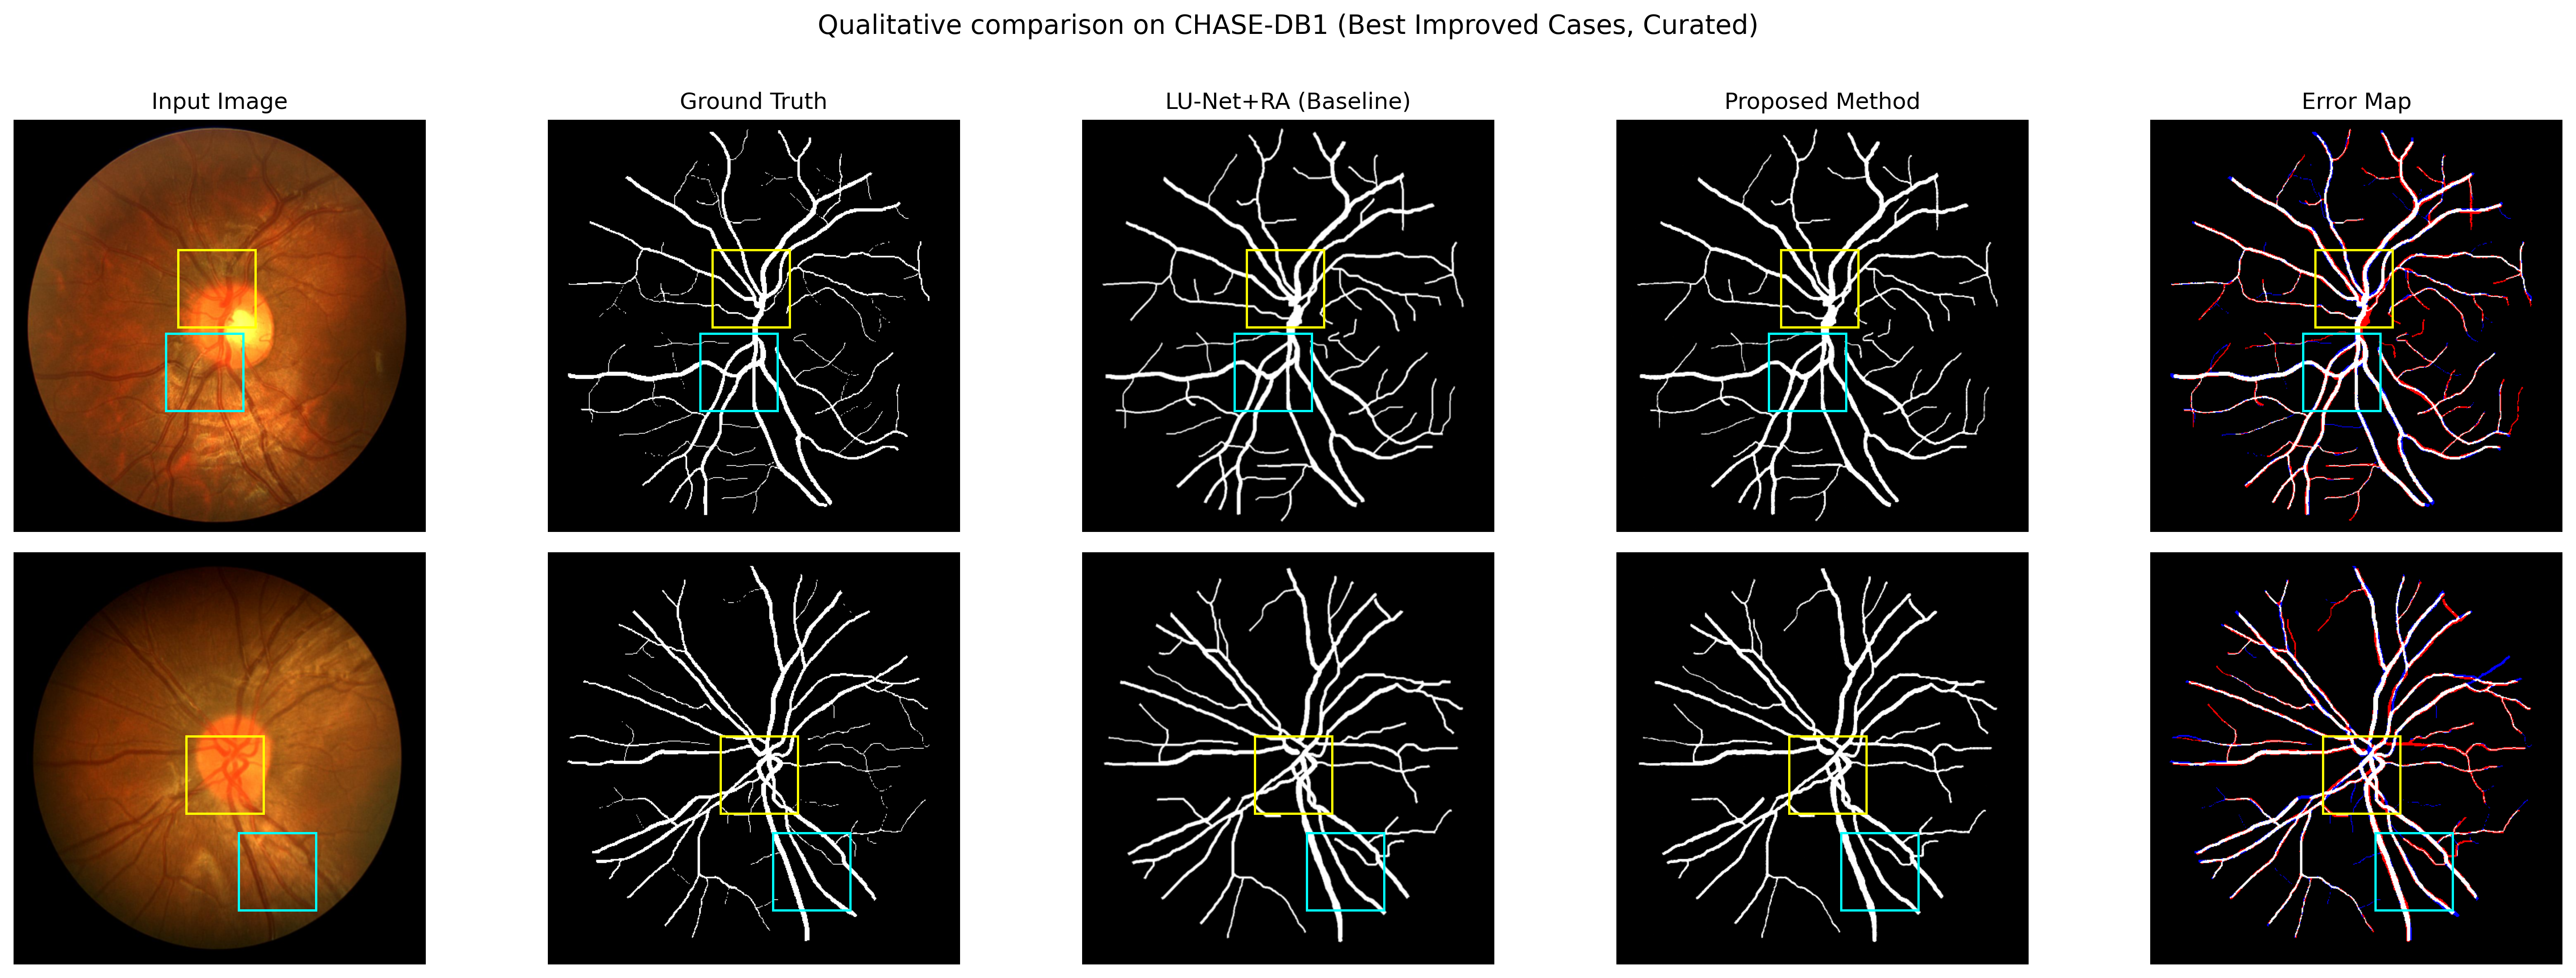
\includegraphics[width=0.98\linewidth,trim=0 0 0 100,clip]{assets/paper2/figure3_qualitative_comparison.png}
\caption{Selected CHASE-DB1 examples \rev{from the earlier single-run experiment} showing the input image, first-observer reference mask, LU-Net+RA coarse prediction, diffusion-refined prediction, and error map for the refined prediction. White, red, blue, and black denote true-positive, false-positive, false-negative, and true-negative pixels, respectively. The examples were selected for visible refinement effects and are illustrative rather than representative.}
\label{fig:qualitative_chase}
\end{figure}

\begin{figure}[htbp]
\centering
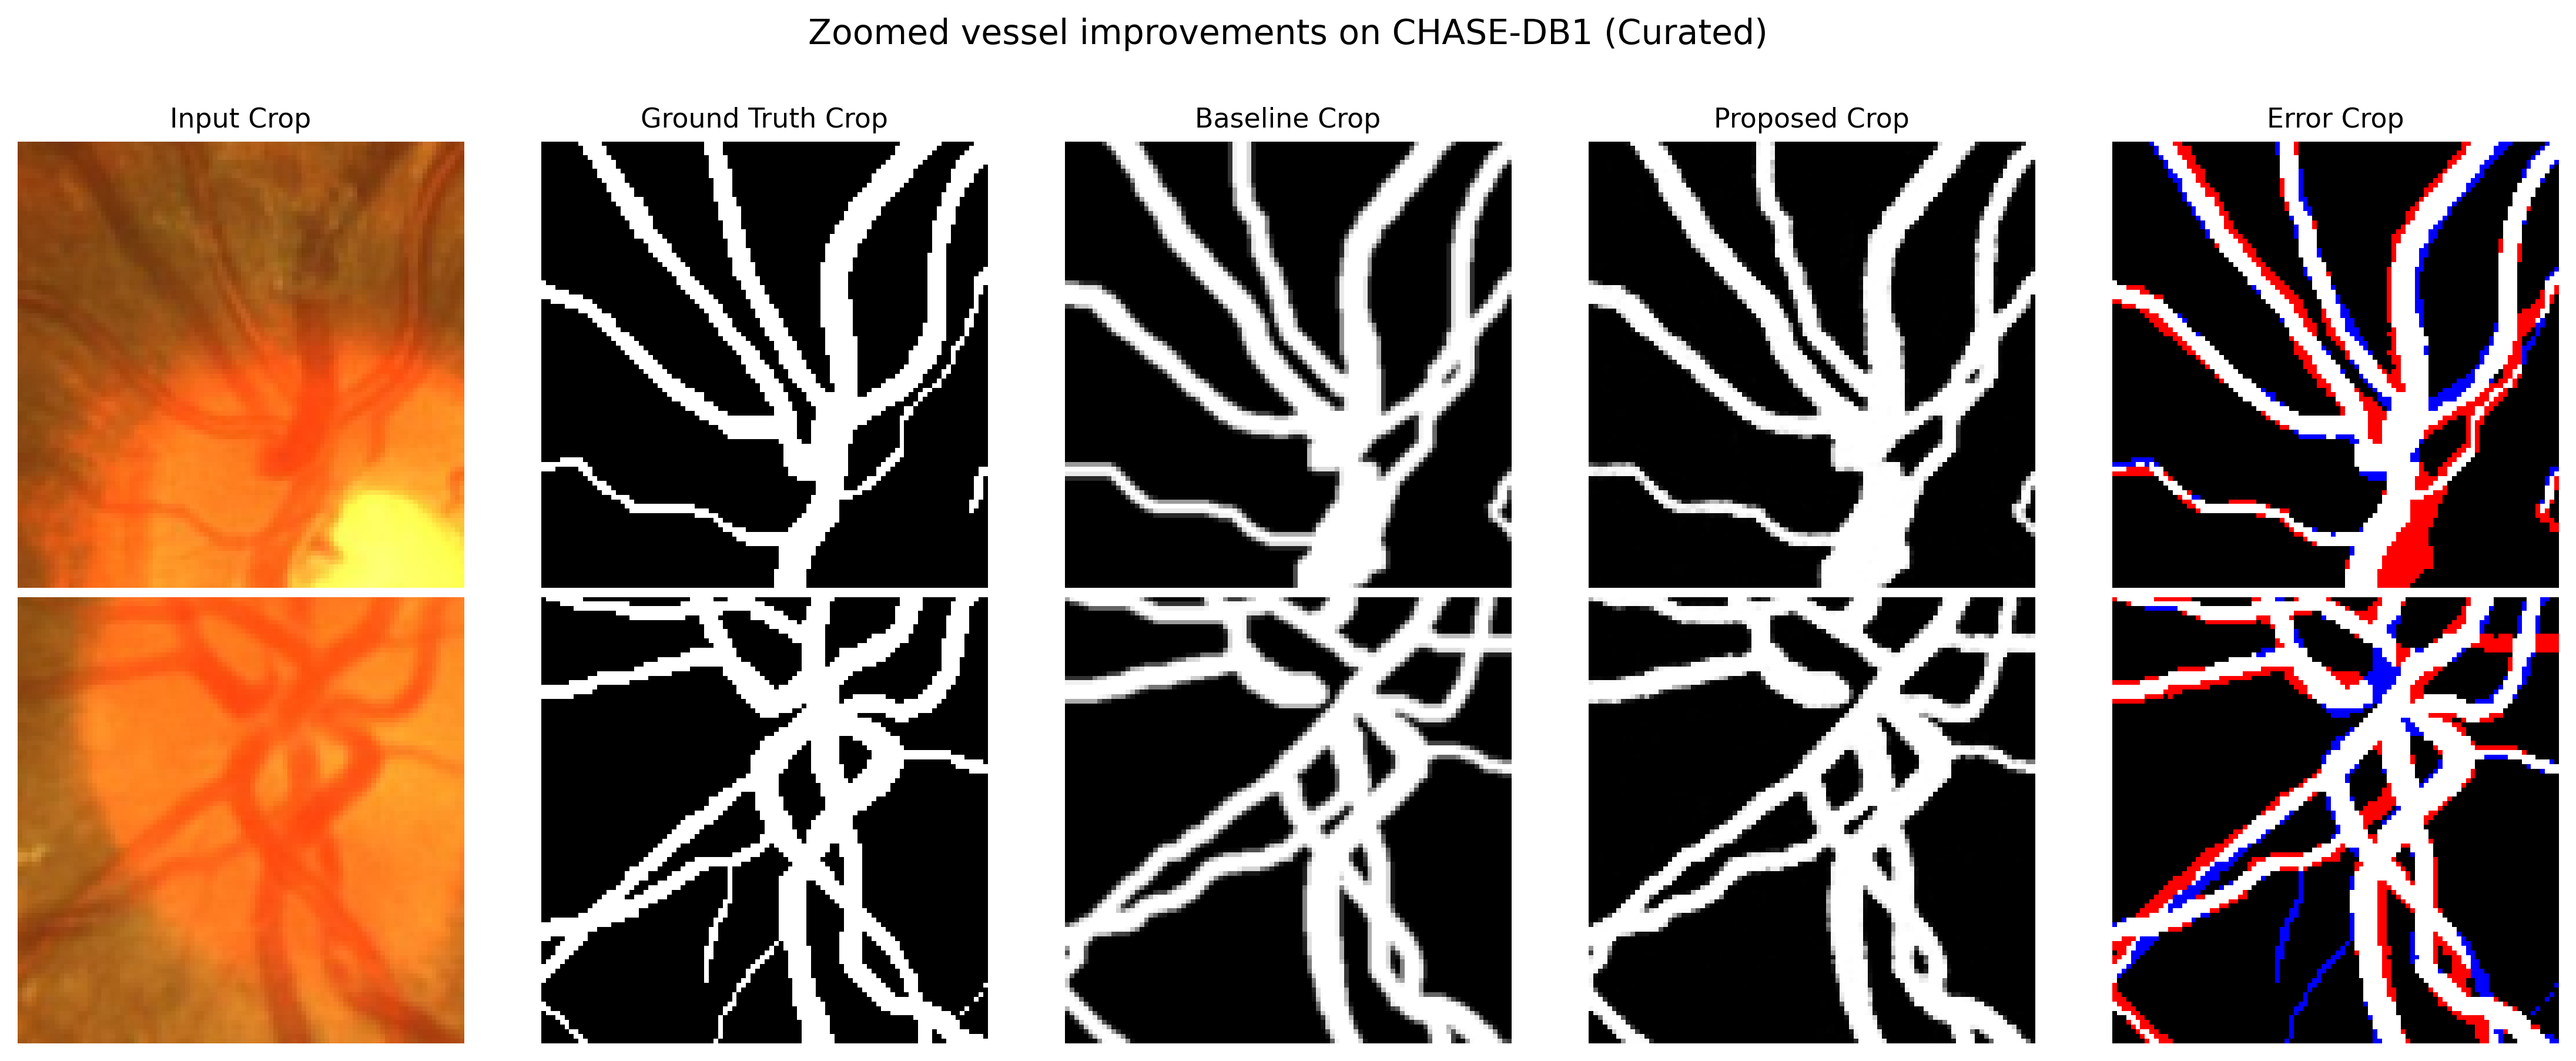
\includegraphics[width=0.98\linewidth,trim=0 0 0 100,clip]{assets/paper2/figure4_zoomed_comparison.png}
\caption{Enlarged regions from selected CHASE-DB1 cases \rev{of the earlier single-run experiment}. Columns show the input crop, first-observer reference mask, LU-Net+RA coarse prediction, diffusion-refined prediction, and refined-prediction error map. White, red, blue, and black denote true-positive, false-positive, false-negative, and true-negative pixels, respectively.}
\label{fig:qualitative_chase_zoom}
\end{figure}

The examples were intentionally selected for visible refinement effects. No inference about average thin-vessel recovery, topology, connectivity, or boundary quality is drawn from these panels; those claims require random or median-case sampling and dedicated centreline, connectivity, or boundary metrics.\secend{qualitative}


\section{Discussion}
\label{sec:discussion}
\seclabel{discussion}

The proposed refiner is most closely related to coarse-to-fine diffusion systems rather than to generic post-processing. HiDiffSeg uses hierarchical vessel and skeleton guidance for retinal segmentation~\cite{HiDiffSeg}; RefineCatDiff incorporates a coarse probability map as prior knowledge in categorical diffusion~\cite{RefineCatDiff}; and the diffusion feature-map denoising module of Li et al.~\cite{DiffusionFMD} is trained end-to-end within existing segmenters. The present design instead performs continuous Gaussian diffusion on an encoded LU-Net+RA probability map, freezes the mask autoencoder, and uses a global RGB condition. These differences motivate the method, but a controlled benchmark is required before claiming an advantage over the related alternatives.

\revbegin{}Under matched partitions, preprocessing, annotations, thresholds and test images, the conditional diffusion refiner lowered mean Dice relative to its own coarse input by 0.064 on CHASE-DB1, 0.002 on DRIVE and 0.066 on HRF (Table~\ref{tab:segmentation_results}). The higher scores of the earlier single-run experiment were not reproduced, and without its checkpoint we cannot determine which configuration differences produced them.

The ablations indicate where the loss arises. Removing the image condition, replacing the global vector with spatial FiLM or using additive injection changed Dice by less than 0.0002, so the global 128-dimensional condition is not the limiting factor in this configuration. Diffusing the encoded reference mask instead of the coarse map gave similar mean Dice from a coarse start and failed from a Gaussian start. A deterministic refiner on the same encoded grid, or joint fine-tuning of the autoencoder, recovered part of the loss, and a spatial residual refiner that bypasses the encoded grid did not lose accuracy and gave small gains on DRIVE and HRF. These patterns are consistent with the frozen, spatially downsampled mask autoencoder limiting the attainable Dice, and show no benefit of the diffusion formulation over deterministic refinement here. We did not measure the reconstruction ceiling of the autoencoder directly, and the spatial refiner also differs in input and augmentation, so this interpretation remains to be tested.

Refinement adds 27\% parameters and raises per-image latency from 4.5~ms for LU-Net+RA to 119~ms for the complete model, and doubling the number of updates doubles refinement time with negligible observed Dice change. Higher Dice alone would not establish better thin-vessel recovery or connectivity, which require topology-aware metrics that we did not evaluate.\secend{discussion}\revend{}

\subsection{Limitations and Reproducibility}
\label{sec:limitations}
\seclabel{limitations}

\revbegin{}The test sets are small: eight CHASE-DB1 images from four subjects, twenty DRIVE images and twelve HRF images, and patient independence is not documented for DRIVE and HRF. Five training seeds give limited statistical resolution; the smallest two-sided exact signed-rank probability is 0.0625, and crossed-bootstrap intervals may under-cover with so few clusters. Holm corrections control each stated family, not all comparisons in the paper. Latency was measured on one GPU. The earlier single-run result could not be verified because its checkpoint and predictions are unavailable.\revend{}

The reference refiner is trained on in-sample backbone predictions; Section~\ref{sec:oof} reports a separate matched OOF comparison. Neither its nonsignificant paired tests nor its exploratory intervals establish equivalence or rule out train--test input shift. Its fold predictors fit fewer images, and the shared frozen DRIVE autoencoder retains in-sample coarse-map pretraining. In addition, its mask autoencoder is pretrained on binary annotations \rev{(for CHASE-DB1 and HRF)} but later encodes soft probability maps. Both choices can create a train-test input shift. The global 128-dimensional image vector also discards spatial conditioning information\rev{, although replacing it with spatial conditioning had negligible effect (Section~\ref{sec:ablations})}. Finally, the $64\times128\times128$ \rev{encoded} grid is spatially coarser than the input mask but contains more scalar values, so the method should not be described as a compressed latent bottleneck.

\rev{We did not reproduce HiDiffSeg, RefineCatDiff or the module of Li et al.\ under our protocol, and we did not run measured ablations of the Dice-loss weight or of refiner augmentation.} The qualitative cases were selected for visible effects, and no centreline, connectivity, boundary, or calibration metric was computed\rev{; we removed the earlier qualitative sampling-variance figure because its sample count and display scale could not be documented, and the manuscript makes no calibration claim}. Future experiments should extend the matched OOF evaluation, use topology-aware metrics, unbiased qualitative sampling and controlled comparisons with recent coarse-to-fine diffusion refiners\rev{, and should test refinement without a frozen, spatially downsampled mask encoding}.\secend{limitations}

%%%%==============================================================


\section{Conclusion}
\label{sec:conclusion}
\seclabel{conclusion}

\revbegin{}We specified and evaluated a conditional diffusion refiner for LU-Net+RA probability maps that operates on a spatially downsampled multi-channel encoding with global RGB conditioning. With five training seeds per configuration and evaluation on the same test images, the refiner did not improve its coarse input: mean Dice was 0.746, 0.790 and 0.666 after refinement, against 0.811, 0.792 and 0.732 for LU-Net+RA on CHASE-DB1, DRIVE and HRF, and an earlier single-run result could not be reproduced. Conditioning variants had negligible effect, deterministic refinement on the same grid and autoencoder fine-tuning recovered part of the loss, and a spatial residual refiner gave small gains on DRIVE and HRF. These results identify the frozen, spatially downsampled mask encoding as a plausible contributor, rather than an isolated cause of the loss, and indicate that any diffusion-specific benefit should be demonstrated against a deterministic refiner under the same protocol. The paired per-image analysis and exploratory intervals are reported in Section~\ref{sec:paired_per_image}; the matched OOF comparison in Section~\ref{sec:oof} does not establish absence of training-input shift.\secend{conclusion}\revend{}
%%%%==============================================================


%\section*{Data Availability Statement}
\dataavailability{CHASE-DB1, DRIVE, and HRF are publicly available from the providers cited in the dataset descriptions~\cite{CHASEDB1,Staal2004,Odstrcilik2013HRF}. \rev{Implementation code and the evaluation and analysis scripts are available at \url{https://github.com/thebabak/Refining_Retinal_Vessel_Segmentation_with_Conditional_Diffusion_Models}. The split files, evaluation records, saved test predictions and model weights are available from the corresponding authors on reasonable request.}}\linelabel{rev:dataavailability}

%\section*{Author Contributions}
%\textit{Contributor Roles Taxonomy (CRediT) statement pending confirmation by all authors before submission.}
\authorcontributions{Conceptualization, H.N. and B.B.; methodology, H.N. and B.B.;
software, B.B.; validation, H.N., B.B. and C.D.; formal analysis, B.B.;
investigation, H.N. and B.B.; resources, H.N. and C.D.; data curation, B.B.;
writing---original draft preparation, B.B.; writing---review and editing, H.N.
and C.D.; visualization, B.B.; supervision, H.N. and C.D.; project
administration, H.N. All authors have read and agreed to the published version
of the manuscript.}

%\section*{Funding}
%\textit{Funding statement pending confirmation by all authors before submission.}
\funding{This research received no external funding.}

%\section*{Institutional Review Board Statement}
\institutionalreview{Not applicable. This computational study used only previously released, de-identified public benchmark datasets and involved no new participant recruitment or data collection.}

%\section*{Informed Consent Statement}
\informedconsent{Not applicable. No new participants were recruited and no new data were collected; consent arrangements for the source datasets were managed by their original providers.}

%\section*{Acknowledgments}
\acknowledgments{During manuscript revision, OpenAI Codex (accessed 15 August 2026) was used for language and structural editing, LaTeX formatting, and reference-consistency checking. The authors reviewed the output and remain responsible for the scientific content, citations, and final submission.}

\conflictsofinterest{The authors declare no conflicts of interest.}
%\section*{Conflicts of Interest}
%\textit{Conflict-of-interest statement pending confirmation by all authors before submission.}

% If authors have a biography, please use the format below
%\section*{Short Biography of Authors}
%\bio
%{\raisebox{-0.35cm}{\includegraphics[width=3.5cm,height=5.3cm,clip,keepaspectratio]{Definitions/author1.pdf}}}
%{\textbf{Firstname Lastname} Biography of first author}
%
%\bio
%{\raisebox{-0.35cm}{\includegraphics[width=3.5cm,height=5.3cm,clip,keepaspectratio]{Definitions/author2.jpg}}}
%{\textbf{Firstname Lastname} Biography of second author}

% For the MDPI journals, use author-date citation, please follow the formatting guidelines on http://www.mdpi.com/authors/references
% To cite two works by the same author: \citeauthor{ref-journal-1a} (\citeyear{ref-journal-1a}, \citeyear{ref-journal-1b}). This produces: Whittaker (1967, 1975)
% To cite two works by the same author with specific pages: \citeauthor{ref-journal-3a} (\citeyear{ref-journal-3a}, p. 328; \citeyear{ref-journal-3b}, p.475). This produces: Wong (1999, p. 328; 2000, p. 475)

%%%%%%%%%%%%%%%%%%%%%%%%%%%%%%%%%%%%%%%%%%
%% for journal Sci
%\reviewreports{\\
%Reviewer 1 comments and authors' response\\
%Reviewer 2 comments and authors' response\\
%Reviewer 3 comments and authors' response
%}
%%%%%%%%%%%%%%%%%%%%%%%%%%%%%%%%%%%%%%%%%%

% =======================
% Manual bibliography
% =======================
\ifmdpiclass
  \reftitle{References}
\else
  \section*{References}
\fi
\begin{thebibliography}{99}

\bibitem{Milletari2016}
Milletari, F.; Navab, N.; Ahmadi, S.-A. V-Net: Fully Convolutional Neural Networks for Volumetric Medical Image Segmentation. In \textit{Proceedings of the 2016 Fourth International Conference on 3D Vision (3DV)}, Stanford, CA, USA, 25--28 October 2016; pp. 565--571. \href{https://doi.org/10.1109/3DV.2016.79}{doi:10.1109/3DV.2016.79}.

\bibitem{Gu2019CENet}
Gu, Z.; Cheng, J.; Fu, H.; Zhou, K.; Hao, H.; Zhao, Y.; Zhang, T.; Gao, S.; Liu, J. CE-Net: Context Encoder Network for 2D Medical Image Segmentation. \textit{IEEE Trans. Med. Imaging} \textbf{2019}, \textit{38}, 2281--2292. \href{https://doi.org/10.1109/TMI.2019.2903562}{doi:10.1109/TMI.2019.2903562}.

\bibitem{Lin2017}
Lin, T.-Y.; Goyal, P.; Girshick, R.; He, K.; Doll\'ar, P. Focal Loss for Dense Object Detection. In \textit{Proceedings of the IEEE International Conference on Computer Vision (ICCV)}, Venice, Italy, 22--29 October 2017; pp. 2980--2988. \href{https://doi.org/10.1109/ICCV.2017.324}{doi:10.1109/ICCV.2017.324}.

\bibitem{Hernandez2025}
Hern\'andez-Guti\'errez, F.D.; Avina-Bravo, E.G.; Ibarra-Manzano, M.A.; Ruiz-Pinales, J.; Ovalle-Magallanes, E.; Avina-Cervantes, J.G. Retinal Vessel Segmentation Based on a Lightweight U-Net and Reverse Attention. \textit{Mathematics} \textbf{2025}, \textit{13}, 2203. \href{https://doi.org/10.3390/math13132203}{doi:10.3390/math13132203}.

\bibitem{Ho2020}
Ho, J.; Jain, A.; Abbeel, P. Denoising Diffusion Probabilistic Models. In \textit{Advances in Neural Information Processing Systems}; Curran Associates: Red Hook, NY, USA, 2020; Volume 33, pp. 6840--6851.

\bibitem{Dhariwal2021}
Dhariwal, P.; Nichol, A. Diffusion Models Beat GANs on Image Synthesis. In \textit{Advances in Neural Information Processing Systems}; Curran Associates: Red Hook, NY, USA, 2021; Volume 34, pp. 8780--8794.

\bibitem{Rombach2022}
Rombach, R.; Blattmann, A.; Lorenz, D.; Esser, P.; Ommer, B. High-Resolution Image Synthesis with Latent Diffusion Models. In \textit{Proceedings of the IEEE/CVF Conference on Computer Vision and Pattern Recognition (CVPR)}, New Orleans, LA, USA, 18--24 June 2022; pp. 10684--10695. \href{https://doi.org/10.1109/CVPR52688.2022.01042}{doi:10.1109/CVPR52688.2022.01042}.

\bibitem{Soares2006}
Soares, J.V.B.; Leandro, J.J.G.; Cesar, R.M., Jr.; Jelinek, H.F.; Cree, M.J. Retinal Vessel Segmentation Using the 2-D Gabor Wavelet and Supervised Classification. \textit{IEEE Trans. Med. Imaging} \textbf{2006}, \textit{25}, 1214--1222. \href{https://doi.org/10.1109/TMI.2006.879967}{doi:10.1109/TMI.2006.879967}.

\bibitem{Mendonca2006}
Mendon\c{c}a, A.M.; Campilho, A. Segmentation of Retinal Blood Vessels by Combining the Detection of Centerlines and Morphological Reconstruction. \textit{IEEE Trans. Med. Imaging} \textbf{2006}, \textit{25}, 1200--1213. \href{https://doi.org/10.1109/TMI.2006.879955}{doi:10.1109/TMI.2006.879955}.

\bibitem{Ronneberger2015}
Ronneberger, O.; Fischer, P.; Brox, T. U-Net: Convolutional Networks for Biomedical Image Segmentation. In \textit{Medical Image Computing and Computer-Assisted Intervention--MICCAI 2015}; Springer: Cham, Switzerland, 2015; LNCS Volume 9351, pp. 234--241. \href{https://doi.org/10.1007/978-3-319-24574-4_28}{doi:10.1007/978-3-319-24574-4\_28}.

\bibitem{Staal2004}
Staal, J.; Abr\`amoff, M.D.; Niemeijer, M.; Viergever, M.A.; van Ginneken, B. Ridge-Based Vessel Segmentation in Color Images of the Retina. \textit{IEEE Trans. Med. Imaging} \textbf{2004}, \textit{23}, 501--509. \href{https://doi.org/10.1109/TMI.2004.825627}{doi:10.1109/TMI.2004.825627}.

\bibitem{Zhou2018UNetpp}
Zhou, Z.; Siddiquee, M.M.R.; Tajbakhsh, N.; Liang, J. UNet++: A Nested U-Net Architecture for Medical Image Segmentation. In \textit{Deep Learning in Medical Image Analysis and Multimodal Learning for Clinical Decision Support}; Springer: Cham, Switzerland, 2018; LNCS Volume 11045, pp. 3--11. \href{https://doi.org/10.1007/978-3-030-00889-5_1}{doi:10.1007/978-3-030-00889-5\_1}.

\bibitem{Oktay2018AttUNet}
Oktay, O.; Schlemper, J.; Le Folgoc, L.; Lee, M.; Heinrich, M.; Misawa, K.; Mori, K.; McDonagh, S.; Hammerla, N.Y.; Kainz, B.; et al. Attention U-Net: Learning Where to Look for the Pancreas. \textit{arXiv} \textbf{2018}, arXiv:1804.03999. \href{https://doi.org/10.48550/arXiv.1804.03999}{doi:10.48550/arXiv.1804.03999}.

\bibitem{Schlemper2019AG}
Schlemper, J.; Oktay, O.; Schaap, M.; Heinrich, M.; Kainz, B.; Glocker, B.; Rueckert, D. Attention Gated Networks: Learning to Leverage Salient Regions in Medical Images. \textit{Med. Image Anal.} \textbf{2019}, \textit{53}, 197--207. \href{https://doi.org/10.1016/j.media.2019.01.012}{doi:10.1016/j.media.2019.01.012}.

\bibitem{Alom2018R2UNet}
Alom, M.Z.; Yakopcic, C.; Hasan, M.; Taha, T.M.; Asari, V.K. Recurrent Residual U-Net for Medical Image Segmentation. \textit{J. Med. Imaging} \textbf{2019}, \textit{6}, 014006. \href{https://doi.org/10.1117/1.JMI.6.1.014006}{doi:10.1117/1.JMI.6.1.014006}.

\bibitem{Liskowski2016}
Liskowski, P.; Krawiec, K. Segmenting Retinal Blood Vessels with Deep Neural Networks. \textit{IEEE Trans. Med. Imaging} \textbf{2016}, \textit{35}, 2369--2380. \href{https://doi.org/10.1109/TMI.2016.2546227}{doi:10.1109/TMI.2016.2546227}.

\bibitem{Fu2016DeepVessel}
Fu, H.; Xu, Y.; Wong, D.W.K.; Liu, J. Retinal Vessel Segmentation via Deep Learning Network and Fully-Connected Conditional Random Fields. In \textit{Proceedings of the 2016 IEEE 13th International Symposium on Biomedical Imaging (ISBI)}, Prague, Czech Republic, 13--16 April 2016; pp. 698--701. \href{https://doi.org/10.1109/ISBI.2016.7493362}{doi:10.1109/ISBI.2016.7493362}.

\bibitem{Shin2019Connectivity}
Shin, S.Y.; Lee, S.; Yun, I.D.; Lee, K.M. Deep Vessel Segmentation by Learning Graphical Connectivity. \textit{Med. Image Anal.} \textbf{2019}, \textit{58}, 101556. \href{https://doi.org/10.1016/j.media.2019.101556}{doi:10.1016/j.media.2019.101556}.

\bibitem{Song2021}
Song, J.; Meng, C.; Ermon, S. Denoising Diffusion Implicit Models. In \textit{Proceedings of the International Conference on Learning Representations}, Virtual, 3--7 May 2021. Available online: \url{https://openreview.net/forum?id=St1giarCHLP} (accessed on 15 August 2026).

\bibitem{Wolleb2022}
Wolleb, J.; Sandk\"uhler, R.; Bieder, F.; Valmaggia, P.; Cattin, P.C. Diffusion Models for Implicit Image Segmentation Ensembles. In \textit{Proceedings of the 5th International Conference on Medical Imaging with Deep Learning}; PMLR: Cambridge, MA, USA, 2022; Volume 172, pp. 1336--1348.

\bibitem{SegDiff}
Amit, T.; Shaharbany, T.; Nachmani, E.; Wolf, L. SegDiff: Image Segmentation with Diffusion Probabilistic Models. \textit{arXiv} \textbf{2021}, arXiv:2112.00390. \href{https://doi.org/10.48550/arXiv.2112.00390}{doi:10.48550/arXiv.2112.00390}.

\bibitem{MedSegDiff}
Wu, J.; Fu, R.; Fang, H.; Zhang, Y.; Yang, Y.; Xiong, H.; Liu, H.; Xu, Y. MedSegDiff: Medical Image Segmentation with Diffusion Probabilistic Model. In \textit{Medical Imaging with Deep Learning}; PMLR: Cambridge, MA, USA, 2024; Volume 227, pp. 1623--1639.

\bibitem{PDDiffusion}
Guo, X.; Yang, Y.; Ye, C.; Lu, S.; Peng, B.; Huang, H.; Xiang, Y.; Ma, T. Accelerating Diffusion Models via Pre-Segmentation Diffusion Sampling for Medical Image Segmentation. In \textit{Proceedings of the 2023 IEEE 20th International Symposium on Biomedical Imaging (ISBI)}, Cartagena, Colombia, 18--21 April 2023. \href{https://doi.org/10.1109/ISBI53787.2023.10230524}{doi:10.1109/ISBI53787.2023.10230524}.

\bibitem{Kazerouni2023}
Kazerouni, A.; Aghdam, E.K.; Heidari, M.; Azad, R.; Fayyaz, M.; Hacihaliloglu, I.; Merhof, D. Diffusion Models in Medical Imaging: A Comprehensive Survey. \textit{Med. Image Anal.} \textbf{2023}, \textit{88}, 102846. \href{https://doi.org/10.1016/j.media.2023.102846}{doi:10.1016/j.media.2023.102846}.

\bibitem{HiDiffSeg}
Huang, W.; Liu, F. HiDiffSeg: A Hierarchical Diffusion Model for Blood Vessel Segmentation in Retinal Fundus Images. \textit{Expert Syst. Appl.} \textbf{2024}, \textit{253}, 124249. \href{https://doi.org/10.1016/j.eswa.2024.124249}{doi:10.1016/j.eswa.2024.124249}.

\bibitem{RefineCatDiff}
Liu, F.; Yu, H.; Huang, J.; Hua, X.; Liu, H.; Ma, Z.; Wang, Z.; Du, Z.; Sun, L. RefineCatDiff: Toward High-Quality Medical Image Segmentation via a Categorical Diffusion Refinement Framework. \textit{Adv. Intell. Syst.} \textbf{2025}, \textit{7}, e202401125. \href{https://doi.org/10.1002/aisy.202401125}{doi:10.1002/aisy.202401125}.

\bibitem{DiffusionFMD}
Li, G.; Jin, D.; Zheng, Y.; Cui, J.; Gai, W.; Qi, M. A Generic Plug \& Play Diffusion-Based Denosing Module for Medical Image Segmentation. \textit{Neural Netw.} \textbf{2024}, \textit{172}, 106096. \href{https://doi.org/10.1016/j.neunet.2024.106096}{doi:10.1016/j.neunet.2024.106096}.

\bibitem{Hu2018}
Hu, J.; Shen, L.; Sun, G. Squeeze-and-Excitation Networks. In \textit{Proceedings of the IEEE/CVF Conference on Computer Vision and Pattern Recognition (CVPR)}, Salt Lake City, UT, USA, 18--23 June 2018; pp. 7132--7141. \href{https://doi.org/10.1109/CVPR.2018.00745}{doi:10.1109/CVPR.2018.00745}.

\bibitem{Woo2018}
Woo, S.; Park, J.; Lee, J.-Y.; Kweon, I.S. CBAM: Convolutional Block Attention Module. In \textit{Computer Vision--ECCV 2018}; Springer: Cham, Switzerland, 2018; LNCS Volume 11211, pp. 3--19. \href{https://doi.org/10.1007/978-3-030-01234-2_1}{doi:10.1007/978-3-030-01234-2\_1}.

\bibitem{Nichol2021}
Nichol, A.Q.; Dhariwal, P. Improved Denoising Diffusion Probabilistic Models. In \textit{Proceedings of the 38th International Conference on Machine Learning}; PMLR: Cambridge, MA, USA, 2021; Volume 139, pp. 8162--8171.

\bibitem{CHASEDB1}
Fraz, M.M.; Remagnino, P.; Hoppe, A.; Uyyanonvara, B.; Rudnicka, A.R.; Owen, C.G.; Barman, S.A. An Ensemble Classification-Based Approach Applied to Retinal Blood Vessel Segmentation. \textit{IEEE Trans. Biomed. Eng.} \textbf{2012}, \textit{59}, 2538--2548. \href{https://doi.org/10.1109/TBME.2012.2205687}{doi:10.1109/TBME.2012.2205687}. Dataset available online: \url{https://researchinnovation.kingston.ac.uk/en/datasets/chasedb1-retinal-vessel-reference-dataset-4/} (accessed on 15 August 2026).

\bibitem{Odstrcilik2013HRF}
Odstr\v{c}il\'{\i}k, J.; Kola\v{r}, R.; Budai, A.; Hornegger, J.; Jan, J.; Gaz\'arek, J.; Kubena, T.; \v{C}ernosek, P.; Svoboda, O.; Angelopoulou, E. Retinal Vessel Segmentation by Improved Matched Filtering: Evaluation on a New High-Resolution Fundus Image Database. \textit{IET Image Process.} \textbf{2013}, \textit{7}, 373--383. \href{https://doi.org/10.1049/iet-ipr.2012.0455}{doi:10.1049/iet-ipr.2012.0455}. Dataset available online: \url{https://www5.cs.fau.de/research/data/fundus-images/} (accessed on 15 August 2026).
\end{thebibliography}

\ifmdpiclass\PublishersNote{}\fi
%\isPreprints{}{% This command is only used for ``preprints''.

%} % If the paper is ``preprints'', please uncomment this parenthesis.
\end{document}
